% future/future.tex
% mainfile: ../perfbook.tex
% SPDX-License-Identifier: CC-BY-SA-3.0

\QuickQuizChapter{chp:Conflicting Visions of the Future}{Conflicting Visions of the Future}{qqzfuture}
%
\Epigraph{Prediction is very difficult, especially about the future.}
	 {\emph{Niels Bohr}}

This chapter presents some conflicting visions of the future of parallel
programming.
It is not clear which of these will come to pass, in fact, it is not
clear that any of them will.
They are nevertheless important because each vision has its devoted
adherents, and if enough people believe in something fervently enough,
you will need to deal with that thing's existence in the form of its
influence on the thoughts, words, and deeds of its adherents.
Besides which, one or more of these visions will actually come to pass.
But most are bogus.
Tell which is which and you'll be rich~\cite{KeithRSpitz1977}!

Therefore, the following sections give an overview of transactional
memory, hardware transactional memory,
formal verification in regression testing, and
parallel functional programming.
But first, a cautionary tale on prognostication taken from the early 2000s.

% future/cpu.tex
% mainfile: ../perfbook.tex
% SPDX-License-Identifier: CC-BY-SA-3.0

\section{The Future of CPU Technology Ain't What it Used to Be}
\label{sec:future:The Future of CPU Technology Ain't What it Used to Be}
%
\epigraph{A great future behind him.}{\emph{David Maraniss}}

Years past always seem so simple and innocent when viewed through the
lens of many years of experience.
And the early 2000s were for the most part innocent of the impending
failure of \IXr{Moore's Law} to continue delivering the then-traditional
increases in CPU clock frequency.
Oh, there were the occasional warnings about the limits of technology,
but such warnings had been sounded for decades.
With that in mind, consider the following scenarios:

\begin{figure}
\centering
\resizebox{3in}{!}{\includegraphics{cartoons/r-2014-CPU-future-uniprocessor-uber-alles}}
\caption{Uniprocessor \"Uber Alles}
\ContributedBy{Figure}{fig:future:Uniprocessor \"Uber Alles}{Melissa Broussard}
\end{figure}

\begin{figure}
\centering
\resizebox{2.6in}{!}{\includegraphics{cartoons/r-2014-CPU-Future-Multithreaded-Mania}}
\caption{Multithreaded Mania}
\ContributedBy{Figure}{fig:future:Multithreaded Mania}{Melissa Broussard}
\end{figure}

\begin{figure}
\centering
\resizebox{2.5in}{!}{\includegraphics{cartoons/r-2014-CPU-Future-More-of-the-Same}}
\caption{More of the Same}
\ContributedBy{Figure}{fig:future:More of the Same}{Melissa Broussard}
\end{figure}

\begin{figure}
\centering
\resizebox{3in}{!}{\includegraphics{cartoons/r-2014-CPU-Future-Crash-dummies}}
\caption{Crash Dummies Slamming into the Memory Wall}
\ContributedBy{Figure}{fig:future:Crash Dummies Slamming into the Memory Wall}{Melissa Broussard}
\end{figure}

\begin{figure}
\centering
\resizebox{3in}{!}{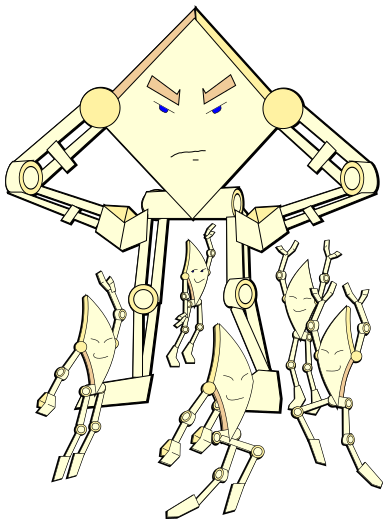
\includegraphics{cartoons/r-2021-CPU-future-astounding-accelerator}}
\caption{Astounding Accelerators}
\ContributedBy{Figure}{fig:future:Astounding Accelerators}{Melissa Broussard, remixed}
\end{figure}

\begin{enumerate}
\item	Uniprocessor \"Uber Alles
	(\cref{fig:future:Uniprocessor \"Uber Alles}),
\item	Multithreaded Mania
	(\cref{fig:future:Multithreaded Mania}),
\item	More of the Same
	(\cref{fig:future:More of the Same}), and
\item	Crash Dummies Slamming into the Memory Wall
	(\cref{fig:future:Crash Dummies Slamming into the Memory Wall}).
\item	Astounding Accelerators
	(\cref{fig:future:Astounding Accelerators}).
\end{enumerate}

Each of these scenarios is covered in the following sections.

\subsection{Uniprocessor \"Uber Alles}
\label{sec:future:Uniprocessor \"Uber Alles}

As was said in 2004~\cite{PaulEdwardMcKenneyPhD}:

\begin{quote}
	In this scenario, the combination of \IXaltr{Moore's-Law}{Moore's Law}
	increases in CPU
	clock rate and continued progress in horizontally scaled computing
	render SMP systems irrelevant.
	This scenario is therefore dubbed ``Uniprocessor \"Uber
	Alles'', literally, uniprocessors above all else.

	These uniprocessor systems would be subject only to instruction
	overhead, since memory barriers, cache thrashing, and contention
	do not affect single-CPU systems.
	In this scenario, RCU is useful only for niche applications, such
	as interacting with \IXacrpl{nmi}.
	It is not clear that an operating system lacking RCU would see
	the need to adopt it, although operating
	systems that already implement RCU might continue to do so.

	However, recent progress with multithreaded CPUs seems to indicate
	that this scenario is quite unlikely.
\end{quote}

Unlikely indeed!
But the larger software community was reluctant to accept the fact that
they would need to embrace parallelism, and so it was some time before
this community concluded that the ``free lunch'' of
\IXaltr{Moore's-Law}{Moore's Law}-induced
CPU core-clock frequency increases was well and truly finished.
Never forget:
Belief is an emotion, not necessarily the result of a rational technical
thought process!

\subsection{Multithreaded Mania}
\label{sec:future:Multithreaded Mania}

Also from 2004~\cite{PaulEdwardMcKenneyPhD}:

\begin{quote}
	A less-extreme variant of Uniprocessor \"Uber Alles features
	uniprocessors with hardware multithreading, and in fact
	multithreaded CPUs are now standard for many desktop and laptop
	computer systems.
	The most aggressively multithreaded CPUs share all levels of
	cache hierarchy, thereby eliminating CPU-to-CPU \IXh{memory}{latency},
	in turn greatly reducing the performance penalty for traditional
	synchronization mechanisms.
	However, a multithreaded CPU would still incur overhead due to
	contention and to pipeline stalls caused by memory barriers.
	Furthermore, because all hardware threads share all levels
	of cache, the cache available to a given hardware thread is a
	fraction of what it would be on an equivalent single-threaded
	CPU, which can degrade performance for applications with large
	cache footprints.
	There is also some possibility that the restricted amount of cache
	available will cause RCU-based algorithms to incur performance
	penalties due to their grace-period-induced additional memory
	consumption.
	Investigating this possibility is future work.

	However, in order to avoid such performance degradation, a number
	of multithreaded CPUs and multi-CPU chips partition at least
	some of the levels of cache on a per-hardware-thread basis.
	This increases the amount of cache available to each hardware
	thread, but re-introduces memory latency for cachelines that
	are passed from one hardware thread to another.
\end{quote}

And we all know how this story has played out, with multiple multi-threaded
cores on a single die plugged into a single socket, with varying degrees
of optimization for lower numbers of active threads per core.
The question then becomes whether or not future shared-memory systems will
always fit into a single socket.

\subsection{More of the Same}
\label{sec:meas:More of the Same}

Again from 2004~\cite{PaulEdwardMcKenneyPhD}:

\begin{quote}
	The More-of-the-Same scenario assumes that the memory-latency
	ratios will remain roughly where they are today.

	This scenario actually represents a change, since to have more
	of the same, interconnect performance must begin keeping up
	with the \IXaltr{Moore's-Law}{Moore's Law} increases in core CPU performance.
	In this scenario, overhead due to pipeline stalls, memory latency,
	and contention remains significant, and RCU retains the high
	level of applicability that it enjoys today.
\end{quote}

And the change has been the ever-increasing levels of integration
that \IXr{Moore's Law} is still providing.
But longer term, which will it be?
More CPUs per die?
Or more I/O, cache, and memory?

Servers seem to be choosing the former, while embedded systems on a chip
(SoCs) continue choosing the latter.

\subsection{Crash Dummies Slamming into the Memory Wall}
\label{sec:future:Crash Dummies Slamming into the Memory Wall}

\begin{figure}
\centering
\epsfxsize=3in
\epsfbox{future/latencytrend}
% from Ph.D. thesis: related/latencytrend.eps
\caption{Instructions per Local Memory Reference for Sequent Computers}
\label{fig:future:Instructions per Local Memory Reference for Sequent Computers}
\end{figure}

\begin{figure}
\centering
\epsfxsize=3in
\epsfbox{future/be-lb-n4-rf-all}
% from Ph.D. thesis: an/plots/be-lb-n4-rf-all.eps
\caption{Breakevens vs.\@ $r$, $\lambda$ Large, Four CPUs}
\label{fig:future:Breakevens vs. r; lambda Large; Four CPUs}
\end{figure}

\begin{figure}
\centering
\epsfxsize=3in
\epsfbox{future/be-lw-n4-rf-all}
% from Ph.D. thesis: an/plots/be-lw-n4-rf-all.eps
\caption{Breakevens vs.\@ $r$, $\lambda$ Small, Four CPUs}
\label{fig:future:Breakevens vs. r; Worst-Case lambda; Four CPUs}
\end{figure}

And one more quote from 2004~\cite{PaulEdwardMcKenneyPhD}:

\begin{quote}
	If the memory-latency trends shown in
	\cref{fig:future:Instructions per Local Memory Reference for Sequent Computers}
	continue, then memory latency will continue to grow relative
	to instruction-execution overhead.
	Systems such as Linux that have significant use of RCU will find
	additional use of RCU to be profitable, as shown in
	\cref{fig:future:Breakevens vs. r; lambda Large; Four CPUs}.
	As can be seen in this figure, if RCU is heavily used, increasing
	memory-latency ratios give RCU an increasing advantage over other
	synchronization mechanisms.
	In contrast, systems with minor
	use of RCU will require increasingly high degrees of read intensity
	for use of RCU to pay off, as shown in
	\cref{fig:future:Breakevens vs. r; Worst-Case lambda; Four CPUs}.
	As can be seen in this figure, if RCU is lightly used,
	increasing memory-latency ratios
	put RCU at an increasing disadvantage compared to other synchronization
	mechanisms.
	Since Linux has been observed with over 1,600 callbacks per \IX{grace
	period} under heavy load~\cite{Sarma04c},
	it seems safe to say that Linux falls into the former category.
\end{quote}

On the one hand, this passage failed to anticipate the cache-warmth
issues that RCU can suffer from in workloads with significant update
intensity, in part because it seemed unlikely that RCU would really
be used for such workloads.
In the event, the \co{SLAB_TYPESAFE_BY_RCU} has been pressed into
service in a number of instances where these cache-warmth issues would
otherwise be problematic, as has sequence locking.
On the other hand, this passage also failed to anticipate that
RCU would be used to reduce scheduling latency or for security.

Much of the data generated for this book was collected on an eight-socket
system with 28 cores per socket and two hardware threads per core, for
a total of 448 hardware threads.
The idle-system memory latencies are less than one microsecond, which
are no worse than those of similar-sized systems of the year 2004.
Some claim that these latencies approach a microsecond only because of
the x86 CPU family's relatively strong memory ordering, but it may be
some time before that particular argument is settled.

\subsection{Astounding Accelerators}
\label{sec:future:Astounding Accelerators}

The potential of hardware accelerators was not quite as clear in 2004
as it is in 2021, so this section has no quote.
However, the November 2020 Top 500 list~\cite{Top500} features a great
many accelerators, so one could argue that this section is a view of
the present rather than of the future.
The same could be said of most of the preceding sections.

Hardware accelerators are being put to many other uses, including
encryption, compression, machine learning.

In short, beware of prognostications, including those in the remainder
of this chapter.

\IfTwoColumn{}{\FloatBarrier}
% future/tm.tex
% mainfile: ../perfbook.tex
% SPDX-License-Identifier: CC-BY-SA-3.0

\section{Transactional Memory}
\label{sec:future:Transactional Memory}
\epigraph{Everything should be as simple as it can be, but not simpler.}
	 {\emph{Albert Einstein, by way of Louis Zukofsky}}

The idea of using transactions outside of databases goes back many
decades~\cite{DBLomet1977SIGSOFT,Knight:1986:AMF:319838.319854,Herlihy93a},
with the key difference between
database and non-database transactions being that non-database transactions
drop the ``D'' in the ``ACID''\footnote{
	Atomicity, consistency, isolation, and durability.}
properties defining database transactions.
The idea of supporting memory-based transactions, or ``transactional memory''
(TM), in hardware
is more recent~\cite{Herlihy93a}, but unfortunately, support for such
transactions in commodity hardware was not immediately forthcoming,
despite other somewhat similar proposals being put forward~\cite{JMStone93}.
Not long after, Shavit and Touitou proposed a software-only implementation
of transactional memory (STM) that was capable of running on commodity
hardware, give or take memory-ordering issues~\cite{Shavit95}.
This proposal languished for many years, perhaps due to the fact that
the research community's attention was absorbed by non-blocking
synchronization (see \cref{sec:advsync:Non-Blocking Synchronization}).

But by the turn of the century, TM started receiving
more attention~\cite{Martinez01a,Rajwar01a}, and by the middle of the
decade, the level of interest can only be termed
``incandescent''~\cite{MauriceHerlihy2005-TM-manifesto.pldi,
DanGrossman2007TMGCAnalogy}, despite a few voices of
caution~\cite{Blundell2005DebunkTM,McKenney2007PLOSTM}.

The basic idea behind TM is to execute a section of
code atomically, so that other threads see no intermediate state.
As such, the semantics of TM could be implemented
by simply replacing each transaction with a recursively acquirable
global lock acquisition and release, albeit with abysmal performance
and scalability.
Much of the complexity inherent in TM implementations, whether hardware
or software, is efficiently detecting when concurrent transactions can safely
run in parallel.
Because this detection is done dynamically, conflicting transactions
can be aborted or ``rolled back'', and in some implementations, this
failure mode is visible to the programmer.

Because transaction roll-back is increasingly unlikely as transaction
size decreases, TM might become quite attractive for small memory-based
operations,
such as linked-list manipulations used for stacks, queues, hash tables,
and search trees.
However, it is currently much more difficult to make the case for large
transactions, particularly those containing non-memory operations such
as I/O and process creation.
The following sections look at current challenges to the grand vision of
``Transactional Memory Everywhere''~\cite{PaulEMcKenney2009TMeverywhere}.
\Cref{sec:future:Outside World} examines the challenges faced
interacting with the outside world,
\cref{sec:future:Process Modification} looks at interactions
with process modification primitives,
\cref{sec:future:Synchronization} explores interactions with
other synchronization primitives, and finally
\cref{sec:future:Discussion} closes with some discussion.

\subsection{Outside World}
\label{sec:future:Outside World}

In the words of Donald Knuth:

\begin{quote}
	Many computer users feel that input and output are not actually part
	of ``real programming,'' they are merely things that (unfortunately)
	must be done in order to get information in and out of the machine.
\end{quote}

Whether we believe that input and output are ``real programming'' or
not, the fact is that for most computer systems, interaction with the
outside world is a first-class requirement.
This section therefore critiques transactional memory's ability to
so interact, whether via I/O operations, time delays, or persistent
storage.

\subsubsection{I/O Operations}
\label{sec:future:I/O Operations}

One can execute I/O operations within a lock-based critical section,
and, at least in principle, from within a userspace-RCU read-side
critical section.
What happens when you attempt to execute an I/O operation from within
a transaction?

The underlying problem is that transactions may be rolled back, for
example, due to conflicts.
Roughly speaking, this requires that all operations within any given
transaction be revocable, so that executing the operation twice has
the same effect as executing it once.
Unfortunately, I/O is in general the prototypical irrevocable
operation, making it difficult to include general I/O operations in
transactions.
In fact, general I/O is irrevocable:
Once you have pushed the button launching the nuclear warheads, there
is no turning back.

Here are some options for handling of I/O within transactions:

\begin{enumerate}
\item	Restrict I/O within transactions to buffered I/O with in-memory
	buffers.
	These buffers may then be included in the transaction in the
	same way that any other memory location might be included.
	This seems to be the mechanism of choice, and it does work
	well in many common cases of situations such as stream I/O and
	mass-storage I/O.
	However, special handling is required in cases where multiple
	record-oriented output streams are merged onto a single file
	from multiple processes, as might be done using the ``a+''
	option to \co{fopen()} or the \co{O_APPEND}  flag to \co{open()}.
	In addition, as will be seen in the next section, common
	networking operations cannot be handled via buffering.
\item	Prohibit I/O within transactions, so that any attempt to execute
	an I/O operation aborts the enclosing transaction (and perhaps
	multiple nested transactions).
	This approach seems to be the conventional TM approach for
	unbuffered I/O, but requires that TM interoperate with other
	synchronization primitives that do tolerate I/O.
\item	Prohibit I/O within transactions, but enlist the compiler's aid
	in enforcing this prohibition.
\item	Permit only one special
	\emph{irrevocable} transaction~\cite{SpearMichaelScott2008InevitableSTM}
	to proceed
	at any given time, thus allowing irrevocable transactions to
	contain I/O operations.\footnote{
		In earlier literature, irrevocable transactions are
		termed \emph{inevitable} transactions.}
	This works in general, but severely limits the scalability and
	performance of I/O operations.
	Given that scalability and performance is a first-class goal of
	parallelism, this approach's generality seems a bit self-limiting.
	Worse yet, use of irrevocability to tolerate I/O operations
	seems to prohibit use of manual transaction-abort operations.\footnote{
		This difficulty was pointed out by Michael Factor.}
	Finally, if there is an irrevocable transaction manipulating
	a given data item, any other transaction manipulating that
	same data item cannot have non-blocking semantics.
\item	Create new hardware and protocols such that I/O operations can
	be pulled into the transactional substrate.
	In the case of input operations, the hardware would need to
	correctly predict the result of the operation, and to abort the
	transaction if the prediction failed.
\end{enumerate}

I/O operations are a well-known weakness of TM, and it is not clear
that the problem of supporting I/O in transactions has a reasonable
general solution, at least if ``reasonable'' is to include usable
performance and scalability.
Nevertheless, continued time and attention to this problem will likely
produce additional progress.

\subsubsection{RPC Operations}
\label{sec:future:RPC Operations}

One can execute RPCs within a lock-based critical section, as well as
from within a userspace-RCU read-side critical section. What happens when you
attempt to execute an RPC from within a transaction?

If both the RPC request and its response are to be contained within the
transaction, and if some part of the transaction depends on the result
returned by the response, then it is not possible to use the memory-buffer
tricks that can be used in the case of buffered I/O.
Any attempt to
take this buffering approach would deadlock the transaction, as the
request could not be transmitted until the transaction was guaranteed
to succeed, but the transaction's success might not be knowable until
after the response is received, as is the case in the following example:

\begin{VerbatimN}
begin_trans();
rpc_request();
i = rpc_response();
a[i]++;
end_trans();
\end{VerbatimN}

The transaction's memory footprint cannot be determined until after the
RPC response is received, and until the transaction's memory footprint
can be determined, it is impossible to determine whether the transaction
can be allowed to commit.
The only action consistent with transactional semantics is therefore to
unconditionally abort the transaction, which is, to say the least,
unhelpful.

Here are some options available to TM:

\begin{enumerate}
\item	Prohibit RPC within transactions, so that any attempt to execute
	an RPC operation aborts the enclosing transaction (and perhaps
	multiple nested transactions).
	Alternatively, enlist the compiler to enforce RPC-free
	transactions.
	This approach does work, but will require TM to
	interact with other synchronization primitives.
\item	Permit only one special
	irrevocable transaction~\cite{SpearMichaelScott2008InevitableSTM}
	to proceed at any given time, thus allowing irrevocable
	transactions to contain RPC operations.
	This works in general, but severely limits the scalability and
	performance of RPC operations.
	Given that scalability and performance is a first-class goal of
	parallelism, this approach's generality seems a bit self-limiting.
	Furthermore, use of irrevocable transactions to permit RPC
	operations rules out manual transaction-abort operations
	once the RPC operation has started.
	Finally, if there is an irrevocable transaction manipulating
	a given data item, any other transaction manipulating that
	same data item cannot have non-blocking semantics.
\item	Identify special cases where the success of the transaction may
	be determined before the RPC response is received, and
	automatically convert these to irrevocable transactions immediately
	before sending the RPC request.
	Of course, if several concurrent transactions attempt RPC calls
	in this manner, it might be necessary to roll all but one of them
	back, with consequent degradation of performance and scalability.
	This approach nevertheless might be valuable given long-running
	transactions ending with an RPC.
	This approach still has problems with manual transaction-abort
	operations.
\item	Identify special cases where the RPC response may be moved out
	of the transaction, and then proceed using techniques similar
	to those used for buffered I/O.
\item	Extend the transactional substrate to include the RPC server as
	well as its client.
	This is in theory possible, as has been demonstrated by
	distributed databases.
	However, it is unclear whether the requisite performance and
	scalability requirements can be met by distributed-database
	techniques, given that memory-based TM cannot hide such latencies
	behind those of slow disk drives.
	Of course, given the advent of solid-state disks, it is also unclear
	how much longer databases will be permitted to hide their latencies
	behind those of disks drives.
\end{enumerate}

As noted in the prior section, I/O is a known weakness of TM, and RPC
is simply an especially problematic case of I/O.

\subsubsection{Time Delays}
\label{sec:future:Time Delays}

An important special case of interaction with extra-transactional accesses
involves explicit time delays within a transaction.
Of course, the idea of a time delay within a transaction flies in the
face of TM's atomicity property, but one can argue that this sort of
thing is what weak atomicity is all about.
Furthermore, correct interaction with memory-mapped I/O sometimes requires
carefully controlled timing, and applications often use time delays
for varied purposes.

So, what can TM do about time delays within transactions?

\begin{enumerate}
\item	Ignore time delays within transactions.
	This has an appearance of elegance, but like too many other
	``elegant'' solutions, fails to survive first contact with
	legacy code.
	Such code, which might well have important time delays in critical
	sections, would fail upon being transactionalized.
\item	Abort transactions upon encountering a time-delay operation.
	This is attractive, but it is unfortunately not always possible
	to automatically detect a time-delay operation.
	Is that tight loop computing something important, or is it
	instead waiting for time to elapse?
\item	Enlist the compiler to prohibit time delays within transactions.
\item	Let the time delays execute normally.
	Unfortunately, some TM implementations publish modifications only
	at commit time, which would in many cases defeat the purpose of
	the time delay.
\end{enumerate}

It is not clear that there is a single correct answer.
TM implementations featuring weak atomicity that publish changes
immediately within the transaction (rolling these changes back upon abort)
might be reasonably well served by the last alternative.
Even in this case, the code (or possibly even hardware) at the other
end of the transaction may require a substantial redesign to tolerate
aborted transactions.
This need for redesign would make it more difficult to apply transactional
memory to legacy code.

\subsubsection{Persistence}
\label{sec:future:Persistence}

There are many different types of locking primitives.
One interesting distinction is persistence, in other words, whether the
lock can exist independently of the address space of the process using
the lock.

Non-persistent locks include \co{pthread_mutex_lock()},
\co{pthread_rwlock_rdlock()}, and most kernel-level locking primitives.
If the memory locations instantiating a non-persistent lock's data
structures disappear, so does the lock.
For typical use of \co{pthread_mutex_lock()}, this means that when the
process exits, all of its locks vanish.
This property can be exploited in order to trivialize lock cleanup
at program shutdown time, but makes it more difficult for unrelated
applications to share locks, as such sharing requires the applications
to share memory.

Persistent locks help avoid the need to share memory among unrelated
applications.
Persistent locking APIs include the flock family, \co{lockf()}, System
V semaphores, or the \co{O_CREAT} flag to \co{open()}.
These persistent APIs can be used to protect large-scale operations
spanning runs of multiple applications, and, in the case of \co{O_CREAT}
even surviving operating-system reboot.
If need be, locks can even span multiple computer systems via distributed
lock managers and distributed filesystems---and persist across reboots
of any or all of these computer systems.

Persistent locks can be used by any application, including applications
written using multiple languages and software environments.
In fact, a persistent lock might well be acquired by an application written
in C and released by an application written in Python.

How could a similar persistent functionality be provided for TM?

\begin{enumerate}
\item	Restrict persistent transactions to special-purpose environments
	designed to support them, for example, SQL.
	This clearly works, given the decades-long history of database
	systems, but does not provide the same degree of flexibility
	provided by persistent locks.
\item	Use snapshot facilities provided by some storage devices and/or
	filesystems.
	Unfortunately, this does not handle network communication,
	nor does it handle I/O to devices that do not provide snapshot
	capabilities, for example, memory sticks.
\item	Build a time machine.
\end{enumerate}

Of course, the fact that it is called transactional \emph{memory}
should give us pause, as the name itself conflicts with the concept of
a persistent transaction.
It is nevertheless worthwhile to consider this possibility as an important
test case probing the inherent limitations of transactional memory.

\subsection{Process Modification}
\label{sec:future:Process Modification}

Processes are not eternal:
They are created and destroyed, their memory mappings are modified,
they are linked to dynamic libraries, and they are debugged.
These sections look at how transactional memory can handle an
ever-changing execution environment.

\subsubsection{Multithreaded Transactions}
\label{sec:future:Multithreaded Transactions}

It is perfectly legal to create processes and threads while holding
a lock or, for that matter, from within a userspace-RCU read-side critical
section.
Not only is it legal, but it is quite simple, as can be seen from the
following code fragment:

\begin{VerbatimN}
pthread_mutex_lock(...);
for (i = 0; i < ncpus; i++)
	pthread_create(&tid[i], ...);
for (i = 0; i < ncpus; i++)
	pthread_join(tid[i], ...);
pthread_mutex_unlock(...);
\end{VerbatimN}

This pseudo-code fragment uses \co{pthread_create()} to spawn one thread
per CPU, then uses \co{pthread_join()} to wait for each to complete,
all under the protection of \co{pthread_mutex_lock()}.
The effect is to execute a lock-based critical section in parallel,
and one could obtain a similar effect using \co{fork()} and \co{wait()}.
Of course, the critical section would need to be quite large to justify
the thread-spawning overhead, but there are many examples of large
critical sections in production software.

What might TM do about thread spawning within a transaction?

\begin{enumerate}
\item	Declare \co{pthread_create()} to be illegal within transactions,
	resulting in transaction abort (preferred) or undefined
	behavior. Alternatively, enlist the compiler to enforce
	\co{pthread_create()}-free transactions.
\item	Permit \co{pthread_create()} to be executed within a
	transaction, but only the parent thread will be considered to
	be part of the transaction.
	This approach seems to be reasonably compatible with existing and
	posited TM implementations, but seems to be a trap for the unwary.
	This approach raises further questions, such as how to handle
	conflicting child-thread accesses.
\item	Convert the \co{pthread_create()}s to function calls.
	This approach is also an attractive nuisance, as it does not
	handle the not-uncommon cases where the child threads communicate
	with one another.
	In addition, it does not permit parallel execution of the body
	of the transaction.
\item	Extend the transaction to cover the parent and all child threads.
	This approach raises interesting questions about the nature of
	conflicting accesses, given that the parent and children are
	presumably permitted to conflict with each other, but not with
	other threads.
	It also raises interesting questions as to what should happen
	if the parent thread does not wait for its children before
	committing the transaction.
	Even more interesting, what happens if the parent conditionally
	executes \co{pthread_join()} based on the values of variables
	participating in the transaction?
	The answers to these questions are reasonably straightforward
	in the case of locking.
	The answers for TM are left as an exercise for the reader.
\end{enumerate}

Given that parallel execution of transactions is commonplace in the
database world, it is perhaps surprising that current TM proposals do
not provide for it.
On the other hand, the example above is a fairly sophisticated use
of locking that is not normally found in simple textbook examples,
so perhaps its omission is to be expected.
That said, there are rumors that some TM researchers are investigating
fork/join parallelism within transactions, so perhaps this topic will
soon be addressed more thoroughly.

\subsubsection{The \tco{exec()} System Call}
\label{sec:future:The exec System Call}

One can execute an \co{exec()} system call while holding a lock, and
also from within an userspace-RCU read-side critical section.
The exact semantics depends on the type of primitive.

In the case of non-persistent primitives (including
\co{pthread_mutex_lock()}, \co{pthread_rwlock_rdlock()}, and userspace RCU),
if the \co{exec()} succeeds, the whole address space vanishes, along
with any locks being held.
Of course, if the \co{exec()} fails, the address space still lives,
so any associated locks would also still live.
A bit strange perhaps, but reasonably well defined.

On the other hand, persistent primitives (including the flock family,
\co{lockf()}, System V semaphores, and the \co{O_CREAT} flag to
\co{open()}) would survive regardless of whether the \co{exec()}
succeeded or failed, so that the \co{exec()}ed program might well
release them.

\QuickQuiz{}
	What about non-persistent primitives represented by data
	structures in \co{mmap()} regions of memory?
	What happens when there is an \co{exec()} within a critical
	section of such a primitive?
\QuickQuizAnswer{
	If the \co{exec()}ed program maps those same regions of
	memory, then this program could in principle simply release
	the lock.
	The question as to whether this approach is sound from a
	software-engineering viewpoint is left as an exercise for
	the reader.
} \QuickQuizEnd

What happens when you attempt to execute an \co{exec()} system call
from within a transaction?

\begin{enumerate}
\item	Disallow \co{exec()} within transactions, so that the enclosing
	transactions abort upon encountering the \co{exec()}.
	This is well defined, but clearly requires non-TM synchronization
	primitives for use in conjunction with \co{exec()}.
\item	Disallow \co{exec()} within transactions, with the compiler
	enforcing this prohibition.
	There is a draft specification for TM in C++ that takes
	this approach, allowing functions to be decorated with
	the \co{transaction_safe} and \co{transaction_unsafe}
	attributes.\footnote{
		Thanks to Mark Moir for pointing me at this spec, and
		to Michael Wong for having pointed me at an earlier
		revision some time back.}
	This approach has some advantages over aborting the transaction
	at runtime, but again requires non-TM synchronization primitives
	for use in conjunction with \co{exec()}.
\item	Treat the transaction in a manner similar to non-persistent
	Locking primitives, so that the transaction survives if \co{exec()}
	fails, and silently commits if the \co{exec()} succeeds.
	The case where some of the variables affected by the transaction
	reside in \co{mmap()}ed memory (and thus could survive a successful
	\co{exec()} system call) is left as an exercise for the reader.
\item	Abort the transaction (and the \co{exec()} system call) if the
	\co{exec()} system call would have succeeded, but allow the
	transaction to continue if the \co{exec()} system call would
	fail.
	This is in some sense the ``correct'' approach, but it would
	require considerable work for a rather unsatisfying result.
\end{enumerate}

The \co{exec()} system call is perhaps the strangest example of an
obstacle to universal TM applicability, as it is not completely clear
what approach makes sense, and some might argue that this is merely a
reflection of the perils of interacting with execs in real life.
That said, the two options prohibiting \co{exec()} within transactions
are perhaps the most logical of the group.

Similar issues surround the \co{exit()} and \co{kill()} system calls,
as well as a \co{longjmp()} or an exception that would exit the transaction.
(Where did the \co{longjmp()} or exception come from?)

\subsubsection{Dynamic Linking and Loading}
\label{sec:future:Dynamic Linking and Loading}

Both lock-based critical sections and userspace-RCU read-side critical sections
can legitimately contain code that invokes dynamically linked and loaded
functions, including C/C++ shared libraries and Java class libraries.
Of course, the code contained in these libraries is by definition
unknowable at compile time.
So, what happens if a dynamically loaded function is invoked within
a transaction?

This question has two parts: (a)~how do you dynamically link and load a
function within a transaction and (b)~what do you do about the unknowable
nature of the code within this function?
To be fair, item (b) poses some challenges for locking and userspace-RCU
as well, at least in theory.
For example, the dynamically linked function might introduce a deadlock
for locking or might (erroneously) introduce a quiescent state into a
userspace-RCU read-side critical section.
The difference is that while the class of operations permitted in locking
and userspace-RCU critical sections is well-understood, there appears
to still be considerable uncertainty in the case of TM.
In fact, different implementations of TM seem to have different restrictions.

So what can TM do about dynamically linked and loaded library functions?
Options for part (a), the actual loading of the code, include the following:

\begin{enumerate}
\item	Treat the dynamic linking and loading in a manner similar to a
	page fault, so that the function is loaded and linked, possibly
	aborting the transaction in the process.
	If the transaction is aborted, the retry will find the function
	already present, and the transaction can thus be expected to
	proceed normally.
\item	Disallow dynamic linking and loading of functions from within
	transactions.
\end{enumerate}

Options for part (b), the inability to detect TM-unfriendly operations
in a not-yet-loaded function, possibilities include the following:

\begin{enumerate}
\item	Just execute the code: if there are any TM-unfriendly operations
	in the function, simply abort the transaction.
	Unfortunately, this approach makes it impossible for the compiler
	to determine whether a given group of transactions may be safely
	composed.
	One way to permit composability regardless is irrevocable
	transactions, however, current implementations permit only a
	single irrevocable transaction to proceed at any given time,
	which can severely limit performance and scalability.
	Irrevocable transactions also seem to rule out use of manual
	transaction-abort operations.
	Finally, if there is an irrevocable transaction manipulating
	a given data item, any other transaction manipulating that
	same data item cannot have non-blocking semantics.
\item	Decorate the function declarations indicating which functions
	are TM-friendly.
	These decorations can then be enforced by the compiler's type system.
	Of course, for many languages, this requires language extensions
	to be proposed, standardized, and implemented, with the
	corresponding time delays.
	That said, the standardization effort is already in
	progress~\cite{Ali-Reza-Adl-Tabatabai2009CppTM}.
\item	As above, disallow dynamic linking and loading of functions from
	within transactions.
\end{enumerate}

I/O operations are of course a known weakness of TM, and dynamic linking
and loading can be thought of as yet another special case of I/O.
Nevertheless, the proponents of TM must either solve this problem, or
resign themselves to a world where TM is but one tool of several in the
parallel programmer's toolbox.
(To be fair, a number of TM proponents have long since resigned themselves
to a world containing more than just TM.)

\subsubsection{Memory-Mapping Operations}
\label{sec:future:Memory-Mapping Operations}

It is perfectly legal to execute memory-mapping operations (including
\co{mmap()}, \co{shmat()}, and \co{munmap()}~\cite{TheOpenGroup1997SUS})
within a lock-based critical section, and, at least in principle, from
within a userspace-RCU read-side critical section.
What happens when you attempt to execute such an operation from within
a transaction?
More to the point, what happens if the memory region being remapped
contains some variables participating in the current thread's transaction?
And what if this memory region contains variables participating in some
other thread's transaction?

It should not be necessary to consider cases where the TM system's
metadata is remapped, given that most locking primitives do not define
the outcome of remapping their lock variables.

Here are some memory-mapping options available to TM:

\begin{enumerate}
\item	Memory remapping is illegal within a transaction, and will result
	in all enclosing transactions being aborted.
	This does simplify things somewhat, but also requires that TM
	interoperate with synchronization primitives that do tolerate
	remapping from within their critical sections.
\item	Memory remapping is illegal within a transaction, and the
	compiler is enlisted to enforce this prohibition.
\item	Memory mapping is legal within a transaction, but aborts all
	other transactions having variables in the region mapped over.
\item	Memory mapping is legal within a transaction, but the mapping
	operation will fail if the region being mapped overlaps with
	the current transaction's footprint.
\item	All memory-mapping operations, whether within or outside a
	transaction, check the region being mapped against the memory
	footprint of all transactions in the system.
	If there is overlap, then the memory-mapping operation fails.
\item	The effect of memory-mapping operations that overlap the memory
	footprint of any transaction in the system is determined by the
	TM conflict manager, which might dynamically determine whether
	to fail the memory-mapping operation or abort any conflicting
	transactions.
\end{enumerate}

It is interesting to note that \co{munmap()} leaves the relevant region
of memory unmapped, which could have additional interesting
implications.\footnote{
	This difference between mapping and unmapping was noted by
	Josh Triplett.}

\subsubsection{Debugging}
\label{sec:future:Debugging}

The usual debugging operations such as breakpoints work normally within
lock-based critical sections and from usespace-RCU read-side critical sections.
However, in initial transactional-memory hardware
implementations~\cite{DaveDice2009ASPLOSRockHTM} an exception within
a transaction will abort that transaction, which in turn means that
breakpoints abort all enclosing transactions.

So how can transactions be debugged?

\begin{enumerate}
\item	Use software emulation techniques within transactions containing
	breakpoints.
	Of course, it might be necessary to emulate all transactions
	any time a breakpoint is set within the scope of any transaction.
	If the runtime system is unable to determine whether or not a
	given breakpoint is within the scope of a transaction, then it
	might be necessary to emulate all transactions just to be on
	the safe side.
	However, this approach might impose significant overhead, which
	might in turn obscure the bug being pursued.
\item	Use only hardware TM implementations that are capable of
	handling breakpoint exceptions.
	Unfortunately, as of this writing (September 2008), all such
	implementations are strictly research prototypes.
\item	Use only software TM implementations, which are
	(very roughly speaking) more tolerant of exceptions than are
	the simpler of the hardware TM implementations.
	Of course, software TM tends to have higher overhead than hardware
	TM, so this approach may not be acceptable in all situations.
\item	Program more carefully, so as to avoid having bugs in the
	transactions in the first place.
	As soon as you figure out how to do this, please do let everyone
	know the secret!
\end{enumerate}

There is some reason to believe that transactional memory will deliver
productivity improvements compared to other synchronization mechanisms,
but it does seem quite possible that these improvements could easily
be lost if traditional debugging techniques cannot be applied to
transactions.
This seems especially true if transactional memory is to be used by
novices on large transactions.
In contrast, macho ``top-gun'' programmers might be able to dispense with
such debugging aids, especially for small transactions.

Therefore, if transactional memory is to deliver on its productivity
promises to novice programmers, the debugging problem does need to
be solved.

\subsection{Synchronization}
\label{sec:future:Synchronization}

If transactional memory someday proves that it can be everything to everyone,
it will not need to interact with any other synchronization mechanism.
Until then, it will need to work with synchronization mechanisms that
can do what it cannot, or that work more naturally in a given situation.
The following sections outline the current challenges in this area.

\subsubsection{Locking}
\label{sec:future:Locking}

It is commonplace to acquire locks while holding other locks, which works
quite well, at least as long as the usual well-known software-engineering
techniques are employed to avoid deadlock.
It is not unusual to acquire locks from within RCU read-side critical
sections, which eases deadlock concerns because RCU read-side primitives
cannot participate in lock-based deadlock cycles.
But what happens when you attempt to acquire a lock from within a transaction?

In theory, the answer is trivial: simply manipulate the data structure
representing the lock as part of the transaction, and everything works
out perfectly.
In practice, a number of non-obvious complications~\cite{Volos2008TRANSACT}
can arise, depending on implementation details of the TM system.
These complications can be resolved, but at the cost of a 45\,\% increase in
overhead for locks acquired outside of transactions and a 300\,\% increase
in overhead for locks acquired within transactions.
Although these overheads might be acceptable for transactional
programs containing small amounts of locking, they are often completely
unacceptable for production-quality lock-based programs wishing to use
the occasional transaction.

\begin{enumerate}
\item	Use only locking-friendly TM implementations.
	Unfortunately, the locking-unfriendly implementations have some
	attractive properties, including low overhead for successful
	transactions and the ability to accommodate extremely large
	transactions.
\item	Use TM only ``in the small'' when introducing TM to lock-based
	programs, thereby accommodating the limitations of
	locking-friendly TM implementations.
\item	Set aside locking-based legacy systems entirely, re-implementing
	everything in terms of transactions.
	This approach has no shortage of advocates, but this requires
	that all the issues described in this series be resolved.
	During the time it takes to resolve these issues, competing
	synchronization mechanisms will of course also have the
	opportunity to improve.
\item	Use TM strictly as an optimization in lock-based systems, as was
	done by the TxLinux~\cite{ChistopherJRossbach2007a} group.
	This approach seems sound, but leaves the locking design
	constraints (such as the need to avoid deadlock) firmly in place.
\item	Strive to reduce the overhead imposed on locking primitives.
\end{enumerate}

The fact that there could possibly be a problem interfacing TM and locking
came as a surprise to many, which underscores the need to try out new
mechanisms and primitives in real-world production software.
Fortunately, the advent of open source means that a huge quantity of
such software is now freely available to everyone, including researchers.

\subsubsection{Reader-Writer Locking}
\label{sec:future:Reader-Writer Locking}

It is commonplace to read-acquire reader-writer locks while holding
other locks, which just works, at least as long as the usual well-known
software-engineering techniques are employed to avoid deadlock.
Read-acquiring reader-writer locks from within RCU read-side critical
sections also works, and doing so eases deadlock concerns because RCU
read-side primitives cannot participate in lock-based deadlock cycles.
But what happens when you attempt to read-acquire a reader-writer lock
from within a transaction?

Unfortunately, the straightforward approach to read-acquiring the
traditional counter-based reader-writer lock within a transaction defeats
the purpose of the reader-writer lock.
To see this, consider a pair of transactions concurrently attempting to
read-acquire the same reader-writer lock.
Because read-acquisition involves modifying the reader-writer lock's
data structures, a conflict will result, which will roll back one of
the two transactions.
This behavior is completely inconsistent with the reader-writer lock's
goal of allowing concurrent readers.

Here are some options available to TM:

\begin{enumerate}
\item	Use per-CPU or per-thread reader-writer
	locking~\cite{WilsonCHsieh92a}, which allows a
	given CPU (or thread, respectively) to manipulate only local
	data when read-acquiring the lock.
	This would avoid the conflict between the two transactions
	concurrently read-acquiring the lock, permitting both to proceed,
	as intended.
	Unfortunately, (1)~the write-acquisition overhead of
	per-CPU/thread locking can be extremely high, (2)~the memory
	overhead of per-CPU/thread locking can be prohibitive, and
	(3)~this transformation is available only when you have access to
	the source code in question.
	Other more-recent scalable
	reader-writer locks~\cite{YossiLev2009SNZIrwlock}
	might avoid some or all of these problems.
\item	Use TM only ``in the small'' when introducing TM to lock-based
	programs, thereby avoiding read-acquiring reader-writer locks
	from within transactions.
\item	Set aside locking-based legacy systems entirely, re-implementing
	everything in terms of transactions.
	This approach has no shortage of advocates, but this requires
	that \emph{all} the issues described in this series be resolved.
	During the time it takes to resolve these issues, competing
	synchronization mechanisms will of course also have the
	opportunity to improve.
\item	Use TM strictly as an optimization in lock-based systems, as was
	done by the TxLinux~\cite{ChistopherJRossbach2007a} group.
	This approach seems sound, but leaves the locking design
	constraints (such as the need to avoid deadlock) firmly in place.
	Furthermore, this approach can result in unnecessary transaction
	rollbacks when multiple transactions attempt to read-acquire
	the same lock.
\end{enumerate}

Of course, there might well be other non-obvious issues surrounding
combining TM with reader-writer locking, as there in fact were with
exclusive locking.

\subsubsection{Deferred Reclamation}
\label{sec:future:Deferred Reclamation}

This section focuses mainly on RCU.
Similar issues and possible resolutions arise when combining TM with
other deferred-reclamation mechanisms such as reference counters and
hazard pointers.
In the text below, known differences are specifically called out.

Because read-copy update (RCU) finds its main use in the Linux kernel,
one might be forgiven for assuming that there had been no academic work
on combining RCU and TM.\footnote{
	However, the in-kernel excuse is wearing thin with the advent
	of user-space RCU~\cite{MathieuDesnoyers2009URCU,MathieuDesnoyers2012URCU}.}
However, the TxLinux group from the University of Texas at Austin had
no choice~\cite{ChistopherJRossbach2007a}.
The fact that they applied TM to the Linux 2.6 kernel, which uses RCU,
forced them to integrate TM and RCU, with TM taking the place of locking
for RCU updates.
Unfortunately, although the paper does state that the RCU implementation's
locks (e.g., \co{rcu_ctrlblk.lock}) were converted to transactions,
it is silent about what happened to locks used in RCU-based updates
(e.g., \co{dcache_lock}).

It is important to note that RCU permits readers and updaters to run
concurrently, further permitting RCU readers to access data that is in
the act of being updated.
Of course, this property of RCU, whatever its performance, scalability,
and real-time-response benefits might be, flies in the face of the
underlying atomicity properties of TM.

So how should TM-based updates interact with concurrent RCU readers?
Some possibilities are as follows:

\begin{enumerate}
\item	RCU readers abort concurrent conflicting TM updates.
	This is in fact the approach taken by the TxLinux project.
	This approach does preserve RCU semantics, and also preserves
	RCU's read-side performance, scalability, and real-time-response
	properties, but it does have the unfortunate side-effect of
	unnecessarily aborting conflicting updates.
	In the worst case, a long sequence of RCU readers could
	potentially starve all updaters, which could in theory result
	in system hangs.
	In addition, not all TM implementations offer the strong atomicity
	required to implement this approach.
\item	RCU readers that run concurrently with conflicting TM updates
	get old (pre-transaction) values from any conflicting RCU loads.
	This preserves RCU semantics and performance, and also prevents
	RCU-update starvation.
	However, not all TM implementations can provide timely access
	to old values of variables that have been tentatively updated
	by an in-flight transaction.
	In particular, log-based TM implementations that maintain
	old values in the log (thus making for excellent TM commit
	performance) are not likely to be happy with this approach.
	Perhaps the \co{rcu_dereference()} primitive can be leveraged
	to permit RCU to access the old values within a greater range
	of TM implementations, though performance might still be an issue.
	Nevertheless, there are popular TM implementations that can
	be easily and efficiently integrated with RCU in this
	manner~\cite{DonaldEPorter2007TRANSACT,PhilHoward2011RCUTMRBTree,
	PhilipWHoward2013RCUrbtree}.
\item	If an RCU reader executes an access that conflicts with an
	in-flight transaction, then that RCU access is delayed until
	the conflicting transaction either commits or aborts.
	This approach preserves RCU semantics, but not RCU's performance
	or real-time response, particularly in presence of long-running
	transactions.
	In addition, not all TM implementations are capable of delaying
	conflicting accesses.
	That said, this approach seems eminently reasonable for hardware
	TM implementations that support only small transactions.
\item	RCU readers are converted to transactions.
	This approach pretty much guarantees that RCU is compatible with
	any TM implementation, but it also imposes TM's rollbacks on RCU
	read-side critical sections, destroying RCU's real-time response
	guarantees, and also degrading RCU's read-side performance.
	Furthermore, this approach is infeasible in cases where any of
	the RCU read-side critical sections contains operations that
	the TM implementation in question is incapable of handling.
	This approach is more difficult to apply to hazard pointers,
	which do not have a sharply defined notion of a reader as
	a section of code.
\item	Many update-side uses of RCU modify a single pointer to publish
	a new data structure.
	In some of these cases, RCU can safely be permitted to see a
	transactional pointer update that is subsequently rolled back,
	as long as the transaction respects memory ordering and as long
	as the roll-back process uses \co{call_rcu()} to free up the
	corresponding structure.
	Unfortunately, not all TM implementations respect memory barriers
	within a transaction.
	Apparently, the thought is that because transactions are supposed
	to be atomic, the ordering of the accesses within the transaction
	is not supposed to matter.
\item	Prohibit use of TM in RCU updates.
	This is guaranteed to work, but seems a bit restrictive.
\end{enumerate}

It seems likely that additional approaches will be uncovered, especially
given the advent of user-level RCU and hazard-pointer
implementations.\footnote{
	Kudos to the TxLinux group, Maged Michael, and Josh Triplett
	for coming up with a number of the above alternatives.}
It is interesting to note that many of the better performing and
scaling STM implementations make use of RCU-like techniques
internally~\cite{KeirAnthonyFraserPhD,KeirFraser2007withoutLocks,Gu:2019:PSE:3358807.3358885}.

\subsubsection{Extra-Transactional Accesses}
\label{sec:future:Extra-Transactional Accesses}

Within a lock-based critical section, it is perfectly legal to manipulate
variables that are concurrently accessed or even modified outside that
lock's critical section, with one common example being statistical
counters.
The same thing is possible within RCU read-side critical
sections, and is in fact the common case.

Given mechanisms such as the so-called ``dirty reads'' that are
prevalent in production database systems, it is not surprising
that extra-transactional accesses have received serious attention
from the proponents of TM, with the concepts of weak and strong
atomicity~\cite{Blundell2006TMdeadlock} being but one case in point.

Here are some extra-transactional options:

\begin{enumerate}
\item	Conflicts due to extra-transactional accesses always abort
	transactions.
	This is strong atomicity.
\item	Conflicts due to extra-transactional accesses are ignored,
	so only conflicts among transactions can abort transactions.
	This is weak atomicity.
\item	Transactions are permitted to carry out non-transactional
	operations in special cases, such as when allocating memory or
	interacting with lock-based critical sections.
\item	Produce hardware extensions that permit some operations
	(for example, addition) to be carried out concurrently on a
	single variable by multiple transactions.
\item	Introduce weak semantics to transactional memory.
	One approach is the combination with RCU described in
	\cref{sec:future:Deferred Reclamation},
	while Gramoli and Guerraoui
	survey a number of other weak-transaction
	approaches~\cite{Gramoli:2014:DTP:2541883.2541900}, for example,
	restricted partitioning of large
	``elastic'' transactions into smaller transactions, thus
	reducing conflict probabilities (albeit with tepid performance
	and scalability).
	Perhaps further experience will show that some uses of
	extra-transactional accesses can be replaced by weak
	transactions.
\end{enumerate}

It appears that transactions were conceived as standing alone, with no
interaction required with any other synchronization mechanism.
If so, it is no surprise that much confusion and complexity arises when
combining transactions with non-transactional accesses.
But unless transactions are to be confined to small updates to isolated
data structures, or alternatively to be confined to new programs
that do not interact with the huge body of existing parallel code,
then transactions absolutely must be so combined if they are to have
large-scale practical impact in the near term.

% @@@ Huge transactions.  Or perhaps conflict handling.

\subsection{Discussion}
\label{sec:future:Discussion}

The obstacles to universal TM adoption lead to the following
conclusions:

\begin{enumerate}
\item	One interesting property of TM is the fact that transactions are
	subject to rollback and retry.
	This property underlies TM's difficulties with irreversible
	operations, including unbuffered I/O, RPCs, memory-mapping
	operations, time delays, and the \co{exec()} system call.
	This property also has the unfortunate consequence of introducing
	all the complexities inherent in the possibility of
	failure into synchronization primitives, often in a developer-visible
	manner.
\item	Another interesting property of TM, noted by
	Shpeisman et al.~\cite{TatianaShpeisman2009CppTM}, is that TM
	intertwines the synchronization with the data it protects.
	This property underlies TM's issues with I/O, memory-mapping
	operations, extra-transactional accesses, and debugging
	breakpoints.
	In contrast, conventional synchronization primitives, including
	locking and RCU, maintain a clear separation between the
	synchronization primitives and the data that they protect.
\item	One of the stated goals of many workers in the TM area is to
	ease parallelization of large sequential programs.
	As such, individual transactions are commonly expected to
	execute serially, which might do much to explain TM's issues
	with multithreaded transactions.
\end{enumerate}

What should TM researchers and developers do about all of this?

One approach is to focus on TM in the small, focusing on situations
where hardware assist potentially provides substantial advantages over
other synchronization primitives.
This is in fact the approach Sun took with its Rock research
CPU~\cite{DaveDice2009ASPLOSRockHTM}.
Some TM researchers seem to agree with this approach, while others have
much higher hopes for TM.

Of course, it is quite possible that TM will be able to take on larger
problems, and this section lists a few of the issues that
must be resolved if TM is to achieve this lofty goal.

Of course, everyone involved should treat this as a learning experience.
It would seem that TM researchers have great deal to learn from
practitioners who have successfully built large software systems using
traditional synchronization primitives.

And vice versa.

\begin{figure}[tb]
\centering
\resizebox{3in}{!}{\includegraphics{cartoons/TM-the-vision}}
\caption{The STM Vision}
\ContributedBy{Figure}{fig:future:The STM Vision}{Melissa Broussard}
\end{figure}

\begin{figure}[tb]
\centering
\resizebox{2.7in}{!}{\includegraphics{cartoons/TM-the-reality-conflict}}
\caption{The STM Reality: Conflicts}
\ContributedBy{Figure}{fig:future:The STM Reality: Conflicts}{Melissa Broussard}
\end{figure}

\begin{figure}[tb]
\centering
\resizebox{3in}{!}{\includegraphics{cartoons/TM-the-reality-nonidempotent}}
\caption{The STM Reality: Irrevocable Operations}
\ContributedBy{Figure}{fig:future:The STM Reality: Irrevocable Operations}{Melissa Broussard}
\end{figure}

\begin{figure}[tb]
\centering
\resizebox{2.7in}{!}{\includegraphics{cartoons/TM-the-reality-realtime}}
\caption{The STM Reality: Realtime Response}
\ContributedBy{Figure}{fig:future:The STM Reality: Realtime Response}{Melissa Broussard}
\end{figure}

But for the moment, the current state of STM
can best be summarized with a series of cartoons.
First,
\cref{fig:future:The STM Vision}
shows the STM vision.
As always, the reality is a bit more nuanced, as fancifully depicted by
\cref{fig:future:The STM Reality: Conflicts,%
fig:future:The STM Reality: Irrevocable Operations,%
fig:future:The STM Reality: Realtime Response}.
Less fanciful STM retrospectives are also
available~\cite{JoeDuffy2010RetroTM,JoeDuffy2010RetroTM2}.

Recent advances in commercially available hardware have opened the door
for variants of HTM, which are addressed in the following section.

\IfTwoColumn{}{\FloatBarrier}
% future/htm.tex

\section{Hardware Transactional Memory}
\label{sec:future:Hardware Transactional Memory}

As of 2017, hardware transactional memory (HTM) is available on several
types of commercially available commodity computer
systems~\cite{Yoo:2013:PEI:2503210.2503232,RickMerrit2011PowerTM,ChristianJacobi2012MainframeTM}.
This section makes a first attempt to find HTM's place in the parallel
programmer's toolbox.

From a conceptual viewpoint, HTM uses processor caches and speculative
execution to make a designated group of statements (a ``transaction'')
take effect atomically
from the viewpoint of any other transactions running on other processors.
This transaction is initiated by a
begin-transaction machine instruction and completed by a commit-transaction
machine instruction.
There is typically also an abort-transaction machine instruction, which
squashes the speculation (as if the begin-transaction instruction and
all following instructions had not executed) and commences execution
at a failure handler.
The location of the failure handler is typically specified by the
begin-transaction instruction, either as an explicit failure-handler
address or via a condition code set by the instruction itself.
Each transaction executes atomically with respect to all other transactions.

HTM has a number of important benefits, including automatic
dynamic partitioning of data structures, reducing synchronization-primitive
cache misses, and supporting a fair number of practical applications.

However, it always pays to read the fine print, and HTM is no exception.
A major point of this section is determining under what conditions HTM's
benefits outweigh the complications hidden in its fine print.
To this end, Section~\ref{sec:future:HTM Benefits WRT to Locking}
describes HTM's benefits and
Section~\ref{sec:future:HTM Weaknesses WRT Locking} describes its weaknesses.
This is the same approach used in earlier
papers~\cite{McKenney2007PLOSTM,PaulEMcKenney2010OSRGrassGreener},
but focused on HTM rather than TM as a whole.\footnote{
	And I gratefully acknowledge many stimulating
	discussions with the other authors, Maged Michael, Josh Triplett,
	and Jonathan Walpole, as well as with Andi Kleen.}

Section~\ref{sec:future:HTM Weaknesses WRT to Locking When Augmented} then describes
HTM's weaknesses with respect to the combination of synchronization
primitives used in the Linux kernel (and in some user-space applications).
Section~\ref{sec:future:Where Does HTM Best Fit In?} looks at where HTM
might best fit into the parallel programmer's toolbox, and
Section~\ref{sec:future:Potential Game Changers} lists some events that might
greatly increase HTM's scope and appeal.
Finally, Section~\ref{sec:future:Conclusions}
presents concluding remarks.

\subsection{HTM Benefits WRT to Locking}
\label{sec:future:HTM Benefits WRT to Locking}

The primary benefits of HTM are
(1)~its avoidance of the cache misses that are often incurred by
other synchronization primitives,
(2)~its ability to dynamically partition
data structures,
and (3)~the fact that it has
a fair number of practical applications.
I break from TM tradition by not listing ease of use separately
for two reasons.
First, ease of use should stem from HTM's primary benefits,
which this section focuses on.
Second, there has been considerable controversy surrounding attempts to
test for raw programming
talent~\cite{RichardBornat2006SheepGoats,SaeedDehnadi2009SheepGoats}
and even around the use of small programming exercises in job
interviews~\cite{RegBraithwaite2007FizzBuzz}.
This indicates that we really do not have a grasp on what makes
programming easy or hard.
Therefore, this section focuses on the three benefits listed above,
each in one of the following sections.

\subsubsection{Avoiding Synchronization Cache Misses}
\label{sec:future:Avoiding Synchronization Cache Misses}

Most synchronization mechanisms are based on data structures that are
operated on by atomic instructions.
Because these atomic instructions normally operate by first causing
the relevant cache line to be owned by the CPU that they are running on,
a subsequent execution
of the same instance of that synchronization primitive on some other
CPU will result in a cache miss.
These communications cache misses severely degrade both the performance and
scalability of conventional synchronization
mechanisms~\cite[Section 4.2.3]{Anderson97}.

In contrast, HTM synchronizes by using the CPU's cache, avoiding the need
for a synchronization data structure and resultant cache misses.
HTM's advantage is greatest in cases where a lock data structure is
placed in a separate cache line, in which case, converting a given
critical section to an HTM transaction can reduce that critical section's
overhead by a full cache miss.
These savings can be quite significant for the common case of short
critical sections, at least for those situations where the elided lock
does not share a cache line with an oft-written variable protected by
that lock.

\QuickQuiz{}
	Why would it matter that oft-written variables shared the cache
	line with the lock variable?
\QuickQuizAnswer{
	If the lock is in the same cacheline as some of the variables
	that it is protecting, then writes to those variables by one CPU
	will invalidate that cache line for all the other CPUs.
	These invalidations will
	generate large numbers of conflicts and retries, perhaps even
	degrading performance and scalability compared to locking.
} \QuickQuizEnd

\subsubsection{Dynamic Partitioning of Data Structures}
\label{sec:future:Dynamic Partitioning of Data Structures}

A major obstacle to the use of some conventional synchronization mechanisms
is the need to statically partition data structures.
There are a number of data structures that are trivially
partitionable, with the most prominent example being hash tables,
where each hash chain constitutes a partition.
Allocating a lock for each hash chain then trivially parallelizes
the hash table for operations confined to a given chain.\footnote{
	And it is also easy to extend this scheme to operations accessing
	multiple hash chains by having such operations acquire the
	locks for all relevant chains in hash order.}
Partitioning is similarly trivial for arrays, radix trees, and a few
other data structures.

However, partitioning for many types of trees and graphs is quite
difficult, and the results are often quite complex~\cite{Ellis80}.
Although it is possible to use two-phased locking and hashed arrays
of locks to partition general data structures, other techniques
have proven preferable~\cite{DavidSMiller2006HashedLocking},
as will be discussed in
Section~\ref{sec:future:HTM Weaknesses WRT to Locking When Augmented}.
Given its avoidance of synchronization cache misses,
HTM is therefore a very real possibility for large non-partitionable
data structures, at least assuming relatively small updates.

\QuickQuiz{}
	Why are relatively small updates important to HTM performance
	and scalability?
\QuickQuizAnswer{
	The larger the updates, the greater the probability of conflict,
	and thus the greater probability of retries, which degrade
	performance.
} \QuickQuizEnd

\subsubsection{Practical Value}
\label{sec:future:Practical Value}

Some evidence of HTM's practical value has been demonstrated in a number
of hardware platforms, including
Sun Rock~\cite{DaveDice2009ASPLOSRockHTM} and
Azul Vega~\cite{CliffClick2009AzulHTM}.
It is reasonable to assume that practical benefits will flow from the
more recent IBM Blue Gene/Q, Intel Haswell TSX, and AMD ASF systems.

Expected practical benefits include:

\begin{enumerate}
\item	Lock elision for in-memory data access and
	update~\cite{Martinez01a,Rajwar02a}.
\item	Concurrent access and small random updates to large non-partitionable
	data structures.
\end{enumerate}

However, HTM also has some very real shortcomings, which will be discussed
in the next section.

\subsection{HTM Weaknesses WRT Locking}
\label{sec:future:HTM Weaknesses WRT Locking}

The concept of HTM is quite simple: A group of accesses and updates to
memory occurs atomically.
However, as is the case with many simple ideas, complications arise
when you apply it to real systems in the real world.
These complications are as follows:

\begin{enumerate}
\item	Transaction-size limitations.
\item	Conflict handling.
\item	Aborts and rollbacks.
\item	Lack of forward-progress guarantees.
\item	Irrevocable operations.
\item	Semantic differences.
\end{enumerate}

Each of these complications is covered in the following sections,
followed by a summary.

\subsubsection{Transaction-Size Limitations}
\label{sec:future:Transaction-Size Limitations}

The transaction-size limitations of current HTM implementations
stem from the use of the processor caches to hold the data
affected by the transaction.
Although this allows a given CPU to make the transaction appear atomic to
other CPUs by executing the transaction within the confines of its cache,
it also means that any transaction that does not fit must be aborted.
Furthermore, events that change execution context, such as interrupts,
system calls, exceptions, traps, and context switches either must
abort any ongoing transaction on the CPU in question or must further
restrict transaction size due to the cache footprint of the other
execution context.

Of course, modern CPUs tend to have large caches, and the data required
for many transactions would fit easily in a one-megabyte cache.
Unfortunately, with caches, sheer size is not all that matters.
The problem is that most caches
can be thought of hash tables implemented in hardware.
However, hardware caches do not chain their buckets (which are normally
called \emph{sets}), but rather
provide a fixed number of cachelines per set.
The number of elements provided for each set in a given cache
is termed that cache's \emph{associativity}.

Although cache associativity varies, the eight-way associativity of
the level-0 cache on the laptop I am typing this on is not unusual.
What this means is that if a given transaction needed to touch
nine cache lines, and if all nine cache lines mapped to the same
set, then that transaction cannot possibly complete, never mind how
many megabytes of additional space might be available in that cache.
Yes, given randomly selected data elements in a given data structure,
the probability of that transaction being able to commit is quite
high, but there can be no guarantee.

There has been some research work to alleviate this limitation.
Fully associative \emph{victim caches} would alleviate the associativity
constraints, but there are currently stringent performance and
energy-efficiency constraints on the sizes of victim caches.
That said, HTM victim caches for unmodified cache lines can be quite
small, as they need to retain only the address:
The data itself can be written to memory or shadowed by other caches,
while the address itself is sufficient to detect a conflicting
write~\cite{RaviRajwar2012TSX}.

\emph{Unbounded transactional memory} (UTM)
schemes~\cite{CScottAnanian2006,KevinEMoore2006}
use DRAM as an extremely large victim cache, but integrating such schemes
into a production-quality cache-coherence mechanism is still an unsolved
problem.
In addition, use of DRAM as a victim cache may have unfortunate
performance and energy-efficiency consequences, particularly
if the victim cache is to be fully associative.
Finally, the ``unbounded'' aspect of UTM assumes that all of DRAM
could be used as a victim cache, while in reality
the large but still fixed amount of DRAM assigned to a given CPU
would limit the size of that CPU's transactions.
Other schemes use a combination of hardware and software transactional
memory~\cite{SanjeevKumar2006} and one could imagine using STM as a
fallback mechanism for HTM.

However, to the best of my knowledge, currently available systems do
not implement any of these research ideas, and perhaps for good reason.

\subsubsection{Conflict Handling}
\label{sec:future:Conflict Handling}

The first complication is the possibility of \emph{conflicts}.
For example, suppose that transactions~A and~B are defined as follows:

\vspace{5pt}
\begin{minipage}[t]{\columnwidth}
\begin{verbatim}
Transaction A       Transaction B

x = 1;              y = 2;
y = 3;              x = 4;
\end{verbatim}
\end{minipage}
\vspace{5pt}

Suppose that each transaction executes concurrently on its own processor.
If transaction~A stores to \co{x} at the same time that transaction~B
stores to \co{y}, neither transaction can progress.
To see this, suppose that transaction~A executes its store to \co{y}.
Then transaction~A will be interleaved within transaction~B, in violation
of the requirement that transactions execute atomically with respect to
each other.
Allowing transaction~B to execute its store to \co{x} similarly violates
the atomic-execution requirement.
This situation is termed a \emph{conflict}, which happens whenever two
concurrent transactions access the same variable where at least one of
the accesses is a store.
The system is therefore obligated to abort one or both of the transactions
in order to allow execution to progress.
The choice of exactly which transaction to abort is an interesting topic
that will very likely retain the ability to generate Ph.D. dissertations for
some time to come, see for
example~\cite{EgeAkpinar2011HTM2TLE}.\footnote{
	Liu's and Spear's paper entitled ``Toxic
	Transactions''~\cite{YujieLiu2011ToxicTransactions} is
	particularly instructive in this regard.}
For the purposes of this section, we can assume that the system makes
a random choice.

Another complication is conflict detection, which is comparatively
straightforward, at least in the simplest case.
When a processor is executing a transaction, it marks every cache line
touched by that transaction.
If the processor's cache receives a request involving a cache line that
has been marked as touched by the current transaction, a potential
conflict has occurred.
More sophisticated systems might try to order the current processors'
transaction to precede that of the processor sending the request,
and optimization of this process will likely also retain the ability
to generate Ph.D. dissertations for quite some time.
However this section assumes a very simple conflict-detection strategy.

However, for HTM to work effectively, the probability of conflict must
be suitably low, which in turn requires that the data structures
be organized so as to maintain a sufficiently low probability of conflict.
For example, a red-black tree with simple insertion, deletion, and search
operations fits this description, but a red-black
tree that maintains an accurate count of the number of elements in
the tree does not.\footnote{
	The need to update the count would result in additions to and
	deletions from the tree conflicting with each other, resulting
	in strong non-commutativity~\cite{HagitAttiya2011LawsOfOrder,Attiya:2011:LOE:1925844.1926442,PaulEMcKenney2011SNC}.}
For another example, a red-black tree that enumerates all elements in
the tree in a single transaction will have high conflict probabilities,
degrading performance and scalability.
As a result, many serial programs will require some restructuring before
HTM can work effectively.
In some cases, practitioners will prefer to take the extra steps
(in the red-black-tree case, perhaps switching to a partitionable
data structure such as a radix tree or a hash table), and just
use locking, particularly during the time before HTM is readily available
on all relevant
architectures~\cite{CliffClick2009AzulHTM}.

\QuickQuiz{}
	How could a red-black tree possibly efficiently enumerate all
	elements of the tree regardless of choice of synchronization
	mechanism???
\QuickQuizAnswer{
	In many cases, the enumeration need not be exact.
	In these cases, hazard pointers or RCU may be used to protect
	readers with low probability of conflict with any given insertion
	or deletion.
} \QuickQuizEnd

Furthermore, the fact that conflicts can occur brings failure handling
into the picture, as discussed in the next section.

\subsubsection{Aborts and Rollbacks}
\label{sec:future:Aborts and Rollbacks}

Because any transaction might be aborted at any time, it is important
that transactions contain no statements that cannot be rolled back.
This means that transactions cannot do I/O, system calls, or debugging
breakpoints (no single stepping in the debugger for HTM transactions!!!).
Instead, transactions must confine themselves to accessing normal
cached memory.
Furthermore, on some systems, interrupts, exceptions, traps,
TLB misses, and other events will also abort transactions.
Given the number of bugs that have resulted from improper handling
of error conditions, it is fair to ask what impact aborts and rollbacks
have on ease of use.

\QuickQuiz{}
	But why can't a debugger emulate single stepping by setting
	breakpoints at successive lines of the transaction, relying
	on the retry to retrace the steps of the earlier instances
	of the transaction?
\QuickQuizAnswer{
	This scheme might work with reasonably high probability, but it
	can fail in ways that would be quite surprising to most users.
	To see this, consider the following transaction:

	\vspace{5pt}
	\begin{minipage}[t]{\columnwidth}
	\small
\begin{verbatim}
  1 begin_trans();
  2 if (a) {
  3   do_one_thing();
  4   do_another_thing();
  5 } else {
  6   do_a_third_thing();
  7   do_a_fourth_thing();
  8 }
  9 end_trans();
\end{verbatim}
	\end{minipage}
	\vspace{5pt}

	Suppose that the user sets a breakpoint at line~3, which triggers,
	aborting the transaction and entering the debugger.
	Suppose that between the time that the breakpoint triggers
	and the debugger gets around to stopping all the threads, some
	other thread sets the value of \co{a} to zero.
	When the poor user attempts to single-step the program, surprise!
	The program is now in the else-clause instead of the then-clause.

	This is \emph{not} what I call an easy-to-use debugger.
} \QuickQuizEnd

Of course, aborts and rollbacks raise the question of whether HTM can
be useful for hard real-time systems.
Do the performance benefits of HTM outweigh the costs of the aborts
and rollbacks, and if so under what conditions?
Can transactions use priority boosting?
Or should transactions for high-priority threads instead preferentially
abort those of low-priority threads?
If so, how is the hardware efficiently informed of priorities?
The literature on real-time use of HTM is quite sparse, perhaps because
researchers are finding more than enough problems in getting
transactions to work well in non-real-time environments.

Because current HTM implementations might deterministically abort a
given transaction, software must provide fallback code.
This fallback code must use some other form of synchronization, for
example, locking.
If the fallback is used frequently, then all the limitations of locking,
including the possibility of deadlock, reappear.
One can of course hope that the fallback isn't used often, which might
allow simpler and less deadlock-prone locking designs to be used.
But this raises the question of how the system transitions from using
the lock-based fallbacks back to transactions.\footnote{
	The possibility of an application getting stuck in fallback
	mode has been termed the ``lemming effect'', a term that
	Dave Dice has been credited with coining.}
One approach is to use a test-and-test-and-set discipline~\cite{Martinez02a},
so that everyone holds off until the lock is released, allowing the
system to start from a clean slate in transactional mode at that point.
However, this could result in quite a bit of spinning, which might not
be wise if the lock holder has blocked or been preempted.
Another approach is to allow transactions to proceed in parallel with
a thread holding a lock~\cite{Martinez02a}, but this raises difficulties
in maintaining atomicity, especially if the reason that the thread is
holding the lock is because the corresponding transaction would not fit
into cache.

Finally, dealing with the possibility of aborts and rollbacks seems to
put an additional burden on the developer, who must correctly handle
all combinations of possible error conditions.

It is clear that users of HTM must put considerable validation effort
into testing both the fallback code paths and transition from fallback
code back to transactional code.

\subsubsection{Lack of Forward-Progress Guarantees}
\label{sec:future:Lack of Forward-Progress Guarantees}

Even though transaction size, conflicts, and aborts/rollbacks can all
cause transactions to abort, one might hope that sufficiently small and
short-duration transactions could be guaranteed to eventually succeed.
This would permit a transaction to be unconditionally retried, in the
same way that compare-and-swap (CAS) and load-linked/store-conditional
(LL/SC) operations are unconditionally retried in code that uses these
instructions to implement atomic operations.

Unfortunately, most currently available HTM implementation refuse to
make any
sort of forward-progress guarantee, which means that HTM cannot be
used to avoid deadlock on those systems.\footnote{
	HTM might well be used to reduce the probability of deadlock,
	but as long as there is some possibility of the fallback
	code being executed, there is some possibility of deadlock.}
Hopefully future implementations of HTM will provide some sort of
forward-progress guarantees.
Until that time, HTM must be used with extreme caution in real-time
applications.\footnote{
	As of mid-2012, there has been surprisingly little work on
	transactional memory's real-time characteristics.}

The one exception to this gloomy picture as of 2013 is upcoming versions
of the IBM mainframe, which provides a separate instruction that may be
used to start a special
\emph{constrained transaction}~\cite{ChristianJacobi2012MainframeTM}.
As you might guess from the name, such transactions must live within
the following constraints:

\begin{enumerate}
\item	Each transaction's data footprint must be contained within
	four 32-byte blocks of memory.
\item	Each transaction is permitted to execute at most 32 assembler
	instructions.
\item	Transactions are not permitted to have backwards branches
	(e.g., no loops).
\item	Each transaction's code is limited to 256 bytes of memory.
\item	If a portion of a given transaction's data footprint resides
	within a given 4K page, then that 4K page is prohibited from
	containing any of that transaction's instructions.
\end{enumerate}

These constraints are severe, but they nevertheless permit a wide variety
of data-structure updates to be implemented, including stacks, queues,
hash tables, and so on.
These operations are guaranteed to eventually complete, and are free of
deadlock and livelock conditions.

It will be interesting to see how hardware support of forward-progress
guarantees evolves over time.

\subsubsection{Irrevocable Operations}
\label{sec:future:Irrevocable Operations}

Another consequence of aborts and rollbacks is that HTM transactions
cannot accommodate irrevocable operations.
Current HTM implementations typically enforce this limitation by
requiring that all of the accesses in the transaction be to cacheable
memory (thus prohibiting MMIO accesses) and aborting transactions on
interrupts, traps, and exceptions (thus prohibiting system calls).

Note that buffered I/O can be accommodated by HTM transactions as
long as the buffer fill/flush operations occur extra-transactionally.
The reason that this works is that adding data to and removing data
from the buffer is revocable: Only the actual buffer fill/flush
operations are irrevocable.
Of course, this buffered-I/O approach has the effect of including the I/O
in the transaction's footprint, increasing the size of the transaction
and thus increasing the probability of failure.

\subsubsection{Semantic Differences}
\label{sec:future:Semantic Differences}

Although HTM can in many cases be used as a drop-in replacement for locking
(hence the name transactional lock
elision~\cite{DaveDice2008TransactLockElision}),
there are subtle differences in semantics.
A particularly nasty example involving coordinated lock-based critical
sections that results in deadlock or livelock when executed transactionally
was given by Blundell~\cite{Blundell2006TMdeadlock}, but a much simpler
example is the empty critical section.

In a lock-based program, an empty critical section will guarantee
that all processes that had previously been holding that lock have
now released it.
This idiom was used by the 2.4 Linux kernel's networking stack to
coordinate changes in configuration.
But if this empty critical section is translated to a transaction,
the result is a no-op.
The guarantee that all prior critical sections have terminated is
lost.
In other words, transactional lock elision preserves the data-protection
semantics of locking, but loses locking's time-based messaging semantics.

\QuickQuiz{}
	But why would \emph{anyone} need an empty lock-based critical
	section???
\QuickQuizAnswer{
	See the answer to \QuickQuizARef{\QlockingQemptycriticalsection} in
	Section~\ref{sec:locking:Exclusive Locks}.

	However, it is claimed that given a strongly atomic HTM
	implementation without forward-progress guarantees, any
	memory-based locking design based on empty critical sections
	will operate correctly in the presence of transactional
	lock elision.
	Although I have not seen a proof of this statement, there
	is a straightforward rationale for this claim.
	The main idea is that in a strongly atomic HTM implementation,
	the results of a given transaction are not visible until
	after the transaction completes successfully.
	Therefore, if you can see that a transaction has started,
	it is guaranteed to have already completed, which means
	that a subsequent empty lock-based critical section will
	successfully ``wait'' on it---after all, there is no waiting
	required.

	This line of reasoning does not apply to weakly atomic
	systems (including many STM implementation), and it also
	does not apply to lock-based programs that use means other
	than memory to communicate.
	One such means is the passage of time (for example, in
	hard real-time systems) or flow of priority (for example,
	in soft real-time systems).

	Locking designs that rely on priority boosting are of particular
	interest.
} \QuickQuizEnd

\QuickQuiz{}
	Can't transactional lock elision trivially handle locking's
	time-based messaging semantics
	by simply choosing not to elide empty lock-based critical sections?
\QuickQuizAnswer{
	It could do so, but this would be both unnecessary and
	insufficient.

	It would be unnecessary in cases where the empty critical section
	was due to conditional compilation.
	Here, it might well be that the only purpose of the lock was to
	protect data, so eliding it completely would be the right thing
	to do.
	In fact, leaving the empty lock-based critical section would
	degrade performance and scalability.

	On the other hand, it is possible for a non-empty lock-based
	critical section to be relying on both the data-protection
	and time-based and messaging semantics of locking.
	Using transactional lock elision in such a case would be
	incorrect, and would result in bugs.
} \QuickQuizEnd

\QuickQuiz{}
	Given modern hardware~\cite{PeterOkech2009InherentRandomness},
	how can anyone possibly expect parallel software relying
	on timing to work?
\QuickQuizAnswer{
	The short answer is that on commonplace commodity hardware,
	synchronization designs based on any sort of fine-grained
	timing are foolhardy and cannot be expected to operate correctly
	under all conditions.

	That said, there are systems designed for hard real-time use
	that are much more deterministic.
	In the (very unlikely) event that you are using such a system,
	here is a toy example showing how time-based synchronization can
	work.
	Again, do \emph{not} try this on commodity microprocessors,
	as they have highly nondeterministic performance characteristics.

	This example uses multiple worker threads along with a control
	thread.
	Each worker thread corresponds to an outbound data feed, and
	records the current time (for example, from the
	\co{clock_gettime()} system call) in a per-thread
	\co{my_timestamp} variable after executing each unit
	of work.
	The real-time nature of this example results in the following
	set of constraints:

	\begin{enumerate}
	\item	It is a fatal error for a given worker thread to fail
		to update its timestamp for a time period of more than
		\co{MAX_LOOP_TIME}.
	\item	Locks are used sparingly to access and update global
		state.
	\item	Locks are granted in strict FIFO order within
		a given thread priority.
	\end{enumerate}

	When worker threads complete their feed, they must disentangle
	themselves from the rest of the application and place a status
	value in a per-thread \co{my_status} variable that is initialized
	to $-1$.
	Threads do not exit; they instead are placed on a thread pool
	to accommodate later processing requirements.
	The control thread assigns (and re-assigns) worker threads as
	needed, and also maintains a histogram of thread statuses.
	The control thread runs at a real-time priority no higher than
	that of the worker threads.

	Worker threads' code is as follows:

	\vspace{5pt}
	\begin{minipage}[t]{\columnwidth}
	\scriptsize
\begin{verbatim}
  1   int my_status = -1;  /* Thread local. */
  2 
  3   while (continue_working()) {
  4     enqueue_any_new_work();
  5     wp = dequeue_work();
  6     do_work(wp);
  7     my_timestamp = clock_gettime(...);
  8   }
  9 
 10   acquire_lock(&departing_thread_lock);
 11 
 12   /*
 13    * Disentangle from application, might
 14    * acquire other locks, can take much longer
 15    * than MAX_LOOP_TIME, especially if many
 16    * threads exit concurrently.
 17    */
 18   my_status = get_return_status();
 19   release_lock(&departing_thread_lock);
 20 
 21   /* thread awaits repurposing. */
\end{verbatim}
	\end{minipage}
	\vspace{5pt}

	The control thread's code is as follows:

	\vspace{5pt}
	\begin{minipage}[t]{\columnwidth}
	\scriptsize
\begin{verbatim}
  1   for (;;) {
  2     for_each_thread(t) {
  3       ct = clock_gettime(...);
  4       d = ct - per_thread(my_timestamp, t);
  5       if (d >= MAX_LOOP_TIME) {
  6         /* thread departing. */
  7         acquire_lock(&departing_thread_lock);
  8         release_lock(&departing_thread_lock);
  9         i = per_thread(my_status, t);
 10         status_hist[i]++; /* Bug if TLE! */
 11       }
 12     }
 13     /* Repurpose threads as needed. */
 14   }
\end{verbatim}
	\end{minipage}
	\vspace{5pt}

	Line~5 uses the passage of time to deduce that the thread
	has exited, executing lines~6-10 if so.
	The empty lock-based critical section on lines~7 and~8
	guarantees that any thread in the process of exiting
	completes (remember that locks are granted in FIFO order!).

	Once again, do not try this sort of thing on commodity
	microprocessors.
	After all, it is difficult enough to get right on systems
	specifically designed for hard real-time use!
} \QuickQuizEnd

One important semantic difference between locking and transactions
is the priority boosting that is used to avoid priority inversion
in lock-based real-time programs.
One way in which priority inversion can occur is when a
low-priority thread holding a lock
is preempted by a medium-priority CPU-bound thread.
If there is at least one such medium-priority thread per CPU, the
low-priority thread will never get a chance to run.
If a high-priority thread now attempts to acquire the lock,
it will block.
It cannot acquire the lock until the low-priority thread releases it,
the low-priority thread cannot release the lock until it gets a chance
to run, and it cannot get a chance to run until one of the medium-priority
threads gives up its CPU.
Therefore, the medium-priority threads are in effect blocking the
high-priority process, which is the rationale for the name ``priority
inversion.''

\begin{figure}[tbp]
{ \scriptsize
\begin{verbbox}
  1 void boostee(void)
  2 {
  3   int i = 0;
  4 
  5   acquire_lock(&boost_lock[i]);
  6   for (;;) {
  7     acquire_lock(&boost_lock[!i]);
  8     release_lock(&boost_lock[i]);
  9     i = i ^ 1;
 10     do_something();
 11   }
 12 }
 13 
 14 void booster(void)
 15 {
 16   int i = 0;
 17 
 18   for (;;) {
 19     usleep(1000); /* sleep 1 ms. */
 20     acquire_lock(&boost_lock[i]);
 21     release_lock(&boost_lock[i]);
 22     i = i ^ 1;
 23   }
 24 }
\end{verbbox}
}
\centering
\theverbbox
\caption{Exploiting Priority Boosting}
\label{fig:future:Exploiting Priority Boosting}
\end{figure}

One way to avoid priority inversion is \emph{priority inheritance},
in which a high-priority thread blocked on a lock temporarily donates
its priority to the lock's holder, which is also called \emph{priority
boosting}.
However, priority boosting can be used for things other than avoiding
priority inversion, as shown in
Figure~\ref{fig:future:Exploiting Priority Boosting}.
Lines~1-12 of this figure show a low-priority process that must
nevertheless run every millisecond or so, while lines~14-24 of
this same figure show a high-priority process that uses priority
boosting to ensure that \co{boostee()} runs periodically as needed.

The \co{boostee()} function arranges this by always holding one of
the two \co{boost_lock[]} locks, so that lines~20-21 of
\co{booster()} can boost priority as needed.

\QuickQuiz{}
	But the \co{boostee()} function in
	Figure~\ref{fig:future:Exploiting Priority Boosting}
	alternatively acquires its locks in reverse order!
	Won't this result in deadlock?
\QuickQuizAnswer{
	No deadlock will result.
	To arrive at deadlock, two different threads must each
	acquire the two locks in oppposite orders, which does not
	happen in this example.
	However, deadlock detectors such as
	lockdep~\cite{JonathanCorbet2006lockdep}
	will flag this as a false positive.
} \QuickQuizEnd

This arrangement requires that \co{boostee()} acquire its first
lock on line~5 before the system becomes busy, but this is easily
arranged, even on modern hardware.

Unfortunately, this arrangement can break down in presence of transactional
lock elision.
The \co{boostee()} function's overlapping critical sections become
one infinite transaction, which will sooner or later abort,
for example, on the first time that the thread running
the \co{boostee()} function is preempted.
At this point, \co{boostee()} will fall back to locking, but given
its low priority and that the quiet initialization period is now
complete (which after all is why \co{boostee()} was preempted),
this thread might never again get a chance to run.

And if the \co{boostee()} thread is not holding the lock, then
the \co{booster()} thread's empty critical section on lines~20 and~21 of
Figure~\ref{fig:future:Exploiting Priority Boosting}
will become an empty transaction that has no effect, so that
\co{boostee()} never runs.
This example illustrates some of the subtle consequences of
transactional memory's rollback-and-retry semantics.

Given that experience will likely uncover additional subtle semantic
differences, application of HTM-based lock elision to large programs
should be undertaken with caution.
That said, where it does apply, HTM-based lock elision can eliminate
the cache misses associated with the lock variable, which has resulted
in tens of percent performance increases in large real-world software
systems as of early 2015.
We can therefore expect to see substantial use of this technique on
hardware supporting it.

\QuickQuiz{}
	So a bunch of people set out to supplant locking, and they
	mostly end up just optimizing locking???
\QuickQuizAnswer{
	At least they accomplished something useful!
	And perhaps there will be additional HTM progress over time.
} \QuickQuizEnd

\subsubsection{Summary}
\label{sec:future:HTM Weaknesses WRT Locking: Summary}

% future/HTMtable.tex
% SPDX-License-Identifier: CC-BY-SA-3.0

\begin{table*}
\centering
% \scriptsize
\small
% future/HTMtableColor.tex
% SPDX-License-Identifier: CC-BY-SA-3.0

\definecolor{plus}{cmyk}{0.1,0,0,0}
\definecolor{minus}{cmyk}{0,0.05,0.2,0.05}
\definecolor{down}{cmyk}{0,0.15,0.15,0.1}
\newcommand{\Pl}{\cellcolor{plus}}
\newcommand{\Mn}{\cellcolor{minus}}
\newcommand{\Dw}{\cellcolor{down}}

\setlength{\tabcolsep}{4pt}\OneColumnHSpace{-.9in}
\ebresizewidth{
\begin{tabularx}{6.5in}{p{0.95in}cXcX}
\toprule
  &
    & \multicolumn{1}{c}{Locking} &
      & \multicolumn{1}{c}{Hardware Transactional Memory} \\
\midrule
  Basic Idea &
    & Allow only one thread at a time to access a given set of objects. &
      & Cause a given operation over a set of objects to execute atomically. \\
\midrule
  Scope &
    & \Pl Handles all operations. &
      & \Pl Handles revocable operations. \\
\addlinespace[4pt]
  &
    & &
      & \Mn Irrevocable operations force fallback (typically to locking). \\
\midrule
  Composability &
    & \Dw Limited by deadlock. &
      & \Dw Limited by irrevocable operations, transaction size,
        and deadlock (assuming lock-based fallback code). \\
\midrule
  Scalability \& Performance &
    & \Mn Data must be partitionable to avoid lock contention. &
      & \Mn Data must be partitionable to avoid conflicts. \\
\cmidrule{3-5}
  &
    & \Dw Partioning must typically be fixed at design time. &
      & \Pl Dynamic adjustment of partitioning carried out automatically down
        to cacheline boundaries. \\
\addlinespace[4pt]
  &
    & &
      & \Mn Partitioning required for fallbacks (less important for rare
        fallbacks). \\
\cmidrule{3-5}
  &
    & \Dw Locking primitives typically result in expensive cache misses
      and memory-barrier instructions. &
      & \Mn Transactions begin/end instructions typically do not result in cache
        misses, but do have memory-ordering and overhead consequences. \\
\cmidrule{3-5}
  &
    & \Pl Contention effects are focused on acquisition and release, so
      that the critical section runs at full speed. &
      & \Mn Contention aborts conflicting transactions, even if they have been
        running for a long time. \\
\cmidrule{3-5}
  &
    & \Pl Privatization operations are simple, intuitive, performant,
      and scalable. &
      & \Mn Privatized data contributes to transaction size. \\
\midrule
  Hardware Support &
    & \Pl Commodity hardware suffices. &
      & \Mn New hardware required (and is starting to become available). \\
\cmidrule{3-5}
  &
    & \Pl Performance is insensitive to cache-geometry details. &
      & \Mn Performance depends critically on cache geometry. \\
\midrule
  Software Support &
    & \Pl APIs exist, large body of code and experience, debuggers operate
      naturally. &
      & \Mn APIs emerging, little experience outside of DBMS, breakpoints
        mid-transaction can be problematic. \\
\midrule
  Interaction With Other Mechanisms &
    & \Pl Long experience of successful interaction. &
      & \Dw Just beginning investigation of interaction. \\
\midrule
  Practical Apps &
    & \Pl Yes. &
      & \Pl Yes. \\
\midrule
  Wide Applicability &
    & \Pl Yes. &
      & \Mn Jury still out. \\
\bottomrule
\end{tabularx}
}
\IfTwoColumn{
\caption{Comparison of Locking and HTM (\colorbox{plus}{Advantage},
  \colorbox{minus}{Disadvantage}, \colorbox{down}{Strong Disadvantage})}
}{
\caption{Comparison of Locking and HTM (\colorbox{plus}{Advantage},
  \colorbox{minus}{Disadvantage},
  \colorbox{down}{Strong} \colorbox{down}{Disadvantage})}
}
\label{tab:future:Comparison of Locking and HTM}
\end{table*}


Although it seems likely that HTM will have compelling use cases,
current implementations have serious transaction-size limitations,
conflict-handling complications, abort-and-rollback issues, and
semantic differences that will require careful handling.
HTM's current situation relative to locking is summarized in
Table~\ref{tab:future:Comparison of Locking and HTM}.
As can be seen, although the current state of HTM alleviates some
serious shortcomings of locking,\footnote{
	In fairness, it is important to emphasize that locking's shortcomings
	do have well-known and heavily used engineering solutions, including
	deadlock detectors~\cite{JonathanCorbet2006lockdep}, a wealth
	of data structures that have been adapted to locking, and
	a long history of augmentation, as discussed in
	Section~\ref{sec:future:HTM Weaknesses WRT to Locking When Augmented}.
	In addition, if locking really were as horrible as a quick skim
	of many academic papers might reasonably lead one to believe,
	where did all the large lock-based parallel programs (both
	FOSS and proprietary) come from, anyway?}
it does so by introducing a significant
number of shortcomings of its own.
These shortcomings are acknowledged by leaders in the TM
community~\cite{AlexanderMatveev2012PessimisticTM}.\footnote{
	In addition, in early 2011, I was invited to deliver a critique of
	some of the assumptions underlying transactional
	memory~\cite{PaulEMcKenney2011Verico}.
	The audience was surprisingly non-hostile, though perhaps they
	were taking it easy on me due to the fact that I was heavily
	jet-lagged while giving the presentation.}

In addition, this is not the whole story.
Locking is not normally used by itself, but is instead typically
augmented by other synchronization mechanisms,
including reference counting, atomic operations, non-blocking data structures,
hazard pointers~\cite{MagedMichael04a,HerlihyLM02},
and RCU~\cite{McKenney98,McKenney01a,ThomasEHart2007a,PaulEMcKenney2012ELCbattery}.
The next section looks at how such augmentation changes the equation.

\subsection{HTM Weaknesses WRT to Locking When Augmented}
\label{sec:future:HTM Weaknesses WRT to Locking When Augmented}

% future/HTMtableRCU.tex
% SPDX-License-Identifier: CC-BY-SA-3.0

\begin{table*}
\centering
\small
% future/HTMtableColor.tex
% SPDX-License-Identifier: CC-BY-SA-3.0

\definecolor{plus}{cmyk}{0.1,0,0,0}
\definecolor{minus}{cmyk}{0,0.05,0.2,0.05}
\definecolor{down}{cmyk}{0,0.15,0.15,0.1}
\newcommand{\Pl}{\cellcolor{plus}}
\newcommand{\Mn}{\cellcolor{minus}}
\newcommand{\Dw}{\cellcolor{down}}

\setstretch{0.95}
\setlength{\tabcolsep}{4pt}\OneColumnHSpace{-.9in}
\ebresizewidth{
\resizebox{6.5in}{!}{
\begin{tabularx}{6.8in}{p{0.95in}cXcX}
\toprule
  &
    & \multicolumn{1}{c}{Locking with Userspace RCU or Hazard Pointers} &
      & \multicolumn{1}{c}{Hardware Transactional Memory} \\
\midrule
  Basic Idea &
    & Allow only one thread at a time to access a given set of objects. &
      & Cause a given operation over a set of objects to execute atomically. \\
\midrule
  Scope &
    & \Pl Handles all operations. &
      & \Pl Handles revocable operations. \\
\addlinespace[4pt]
  &
    & &
      & \Mn Irrevocable operations force fallback (typically to locking). \\
\midrule
  Composability &
    & \Pl Readers limited only by grace-period-wait operations. &
      & \Dw Limited by irrevocable operations, transaction size, and deadlock.
        (Assuming lock-based fallback code.)\\
\addlinespace[4pt]
  &
    & \Mn Updaters limited by deadlock.  Readers reduce deadlock. &
      & \\
\midrule
  Scalability \& Performance &
    & \Mn Data must be partitionable to avoid lock contention among updaters. &
      & \Mn Data must be partitionable to avoid conflicts. \\
\addlinespace[4pt]
  &
    & \Pl Partitioning not needed for readers. &
      & \\
\cmidrule{3-5}
  &
    & \Dw Partitioning for updaters must typically be fixed at design time. &
      & \Pl Dynamic adjustment of partitioning carried out automatically down
        to cacheline boundaries. \\
\cmidrule{3-5}
  &
    & \Pl Partitioning not needed for readers. &
      & \Mn Partitioning required for fallbacks (less important for rare
        fallbacks). \\
\cmidrule{3-5}
  &
    & \Dw Updater locking primitives typically result in expensive cache misses
      and memory-barrier instructions. &
      & \Mn Transactions begin/end instructions typically do not result in
        cache misses, but do have memory-ordering and overhead consequences. \\
\cmidrule{3-5}
  &
    & \Pl Update-side contention effects are focused on acquisition and release,
      so that the critical section runs at full speed. &
      & \Mn Contention aborts conflicting transactions, even if they have been
        running for a long time. \\
\addlinespace[4pt]
  &
    & \Pl Readers do not contend with updaters or with each other. &
      & \\
\cmidrule{3-5}
  &
    & \Pl Read-side primitives are typically bounded wait-free with low
      overhead.
      (Lock-free with low overhead for hazard pointers.) &
      & \Mn Read-only transactions subject to conflicts and rollbacks.
        No forward-progress guarantees other than those supplied by fallback
        code. \\
\cmidrule{3-5}
  &
    & \Pl Privatization operations are simple, intuitive, performant, and
      scalable when data is visible only to updaters. &
      & \Mn Privatized data contributes to transaction size. \\
\addlinespace[4pt]
  &
    & \Mn Privatization operations are expensive (though still intuitive
      and scalable) for reader-visible data. &
      & \\
\midrule
  Hardware Support &
    & \Pl Commodity hardware suffices. &
      & \Mn New hardware required (and is starting to become available). \\
\cmidrule{3-5}
  &
    & \Pl Performance is insensitive to cache-geometry details. &
      & \Mn Performance depends critically on cache geometry. \\
\midrule
  Software Support &
    & \Pl APIs exist, large body of code and experience, debuggers operate
      naturally. &
      & \Mn APIs emerging, little experience outside of DBMS, breakpoints
        mid-transaction can be problematic. \\
\midrule
  Interaction With Other Mechanisms &
    & \Pl Long experience of successful interaction. &
      & \Dw Just beginning investigation of interaction. \\
\midrule
  Practical Apps &
    & \Pl Yes. &
      & \Pl Yes. \\
\midrule
  Wide Applicability &
    & \Pl Yes. &
      & \Mn Jury still out. \\
\bottomrule
\end{tabularx}
}}
\caption{Comparison of Locking (Augmented by RCU or Hazard Pointers) and HTM
  (\colorbox{plus}{Advantage}, \colorbox{minus}{Disadvantage},
  \colorbox{down}{Strong Disadvantage})}
\label{tab:future:Comparison of Locking (Augmented by RCU or Hazard Pointers) and HTM}
\end{table*}


Practitioners have long used reference counting, atomic operations,
non-blocking data structures, hazard pointers, and RCU to avoid some
of the shortcomings of locking.
For example, deadlock can be avoided in many cases by using reference
counts, hazard pointers, or RCU to protect data structures,
particularly for read-only critical
sections~\cite{MagedMichael04a,HerlihyLM02,MathieuDesnoyers2012URCU,DinakarGuniguntala2008IBMSysJ,ThomasEHart2007a}.
These approaches also reduce the need to partition data
structures, as was see in Chapter~\ref{chp:Data Structures}.
RCU further provides contention-free wait-free read-side
primitives~\cite{MathieuDesnoyers2012URCU}.
Adding these considerations to
Table~\ref{tab:future:Comparison of Locking and HTM}
results in the updated comparison between augmented locking and HTM
shown in
Table~\ref{tab:future:Comparison of Locking (Augmented by RCU or Hazard Pointers) and HTM}.
A summary of the differences between the two tables is as follows:

\begin{enumerate}
\item	Use of non-blocking read-side mechanisms alleviates deadlock issues.
\item	Read-side mechanisms such as hazard pointers and RCU can operate
	efficiently on non-partitionable data.
\item	Hazard pointers and RCU do not contend with each other or with
	updaters, allowing excellent performance and scalability for
	read-mostly workloads.
\item	Hazard pointers and RCU provide forward-progress guarantees
	(lock freedom and wait-freedom, respectively).
\item	Privatization operations for hazard pointers and RCU are
	straightforward.
\end{enumerate}

Of course, it is also possible to augment HTM,
as discussed in the next section.

\subsection{Where Does HTM Best Fit In?}
\label{sec:future:Where Does HTM Best Fit In?}

Although it will likely be some time before HTM's area of applicability
can be as crisply delineated as that shown for RCU in
Figure~\ref{fig:defer:RCU Areas of Applicability} on
page~\pageref{fig:defer:RCU Areas of Applicability}, that is no reason not to
start moving in that direction.

HTM seems best suited to update-heavy workloads involving relatively
small changes to disparate portions of relatively large in-memory
data structures running on large multiprocessors,
as this meets the size restrictions of current HTM implementations while
minimizing the probability of conflicts and attendant aborts and
rollbacks.
This scenario is also one that is relatively difficult to handle given
current synchronization primitives.

Use of locking in conjunction with HTM seems likely to overcome HTM's
difficulties with irrevocable operations, while use of RCU or
hazard pointers might alleviate HTM's transaction-size limitations
for read-only operations that traverse large fractions of the data
structure.
Current HTM implementations unconditionally abort an update transaction
that conflicts with an RCU or hazard-pointer reader, but perhaps future
HTM implementations will interoperate more smoothly with these
synchronization mechanisms.
In the meantime, the probability of an update conflicting with a
large RCU or hazard-pointer read-side critical section should be
much smaller than the probability of conflicting with the equivalent
read-only transaction.\footnote{
	It is quite ironic that strictly transactional mechanisms are
	appearing in shared-memory systems at just about the time
	that NoSQL databases are relaxing the traditional
	database-application reliance on strict transactions.}
Nevertheless, it is quite possible that a steady stream of RCU or
hazard-pointer readers might starve updaters due to a corresponding
steady stream of conflicts.
This vulnerability could be eliminated (perhaps at significant
hardware cost and complexity) by giving extra-transactional
reads the pre-transaction copy of the memory location being loaded.

The fact that HTM transactions must have fallbacks might in some cases
force static partitionability of data structures back onto HTM.
This limitation might be alleviated if future HTM implementations
provide forward-progress guarantees, which might eliminate the need
for fallback code in some cases, which in turn might allow HTM to
be used efficiently in situations with higher conflict probabilities.

In short, although HTM is likely to have important uses and applications,
it is another tool in the parallel programmer's toolbox, not a replacement
for the toolbox in its entirety.

\subsection{Potential Game Changers}
\label{sec:future:Potential Game Changers}

Game changers that could greatly increase the need for HTM include
the following:

\begin{enumerate}
\item	Forward-progress guarantees.
\item	Transaction-size increases.
\item	Improved debugging support.
\item	Weak atomicity.
\end{enumerate}

These are expanded upon in the following sections.

\subsubsection{Forward-Progress Guarantees}
\label{sec:future:Forward-Progress Guarantees}

As was discussed in
Section~\ref{sec:future:Lack of Forward-Progress Guarantees},
current HTM implementations lack forward-progress guarantees, which requires
that fallback software be available to handle HTM failures.
Of course, it is easy to demand guarantees, but not always easy
to provide them.
In the case of HTM, obstacles to guarantees can include cache size and
associativity, TLB size and associativity, transaction duration and
interrupt frequency, and scheduler implementation.

Cache size and associativity was discussed in
Section~\ref{sec:future:Transaction-Size Limitations},
along with some research intended to work around current limitations.
However, HTM forward-progress guarantees would
come with size limits, large though these limits might one day be.
So why don't current HTM implementations provide forward-progress
guarantees for small transactions, for example, limited to the
associativity of the cache?
One potential reason might be the need to deal with hardware failure.
For example, a failing cache SRAM cell might be handled by deactivating
the failing cell, thus reducing the associativity of the cache and
therefore also the maximum size of transactions that can be guaranteed
forward progress.
Given that this would simply decrease the guaranteed transaction size,
it seems likely that other reasons are at work.
Perhaps providing forward progress guarantees on production-quality
hardware is more difficult than one might think, an entirely plausible
explanation given the difficulty of making forward-progress guarantees
in software.
Moving a problem from software to hardware does not necessarily make
it easier to solve.

Given a physically tagged and indexed cache, it is not enough for the
transaction to fit in the cache.
Its address translations must also fit in the TLB.
Any forward-progress guarantees must therefore also take TLB size
and associativity into account.

Given that interrupts, traps, and exceptions abort transactions in current
HTM implementations, it is necessary that the execution duration of
a given transaction be shorter than the expected interval between
interrupts.
No matter how little data a given transaction touches, if it runs too
long, it will be aborted.
Therefore, any forward-progress guarantees must be conditioned not only
on transaction size, but also on transaction duration.

Forward-progress guarantees depend critically on the ability to determine
which of several conflicting transactions should be aborted.
It is all too easy to imagine an endless series of transactions, each
aborting an earlier transaction only to itself be aborted by a later
transactions, so that none of the transactions actually commit.
The complexity of conflict handling is
evidenced by the large number of HTM conflict-resolution policies
that have been proposed~\cite{EgeAkpinar2011HTM2TLE,YujieLiu2011ToxicTransactions}.
Additional complications are introduced by extra-transactional accesses,
as noted by Blundell~\cite{Blundell2006TMdeadlock}.
It is easy to blame the extra-transactional accesses for all of these
problems, but the folly of this line of thinking is easily demonstrated
by placing each of the extra-transactional accesses into its own
single-access transaction.
It is the pattern of accesses that is the issue, not whether or not they
happen to be enclosed in a transaction.

Finally, any forward-progress guarantees for transactions also
depend on the scheduler, which must let the thread executing the
transaction run long enough to successfully commit.

So there are significant obstacles to HTM vendors offering forward-progress
guarantees.
However, the impact of any of them doing so would be enormous.
It would mean that HTM transactions would no longer need software
fallbacks, which would mean that HTM could finally deliver on the
TM promise of deadlock elimination.

And as of late 2012, the IBM Mainframe announced an HTM
implementation that includes \emph{constrained transactions}
in addition to the usual best-effort HTM
implementation~\cite{ChristianJacobi2012MainframeTM}.
A constrained transaction starts with the \co{tbeginc} instruction
instead of the \co{tbegin} instruction that is used for best-effort
transactions.
Constrained transactions are guaranteed to always complete (eventually),
so if a transaction aborts, rather than branching to a fallback path
(as is done for best-effort transactions), the hardware instead restarts
the transaction at the \co{tbeginc} instruction.

The Mainframe architects needed to take extreme measures to deliver on
this forward-progress guarantee.
If a given constrained transaction repeatedly fails, the CPU
might disable branch prediction, force in-order execution, and even
disable pipelining.
If the repeated failures are due to high contention, the CPU might
disable speculative fetches, introduce random delays, and even
serialize execution of the conflicting CPUs.
``Interesting'' forward-progress scenarios involve as few as two CPUs
or as many as one hundred CPUs.
Perhaps these extreme measures provide some insight as to why other CPUs
have thus far refrained from offering constrained transactions.

As the name implies, constrained transactions are in fact severely constrained:

\begin{enumerate}
\item	The maximum data footprint is four blocks of memory,
	where each block can be no larger than 32 bytes.
\item	The maximum code footprint is 256 bytes.
\item	If a given 4K page contains a constrained transaction's code,
	then that page may not contain that transaction's data.
\item	The maximum number of assembly instructions that may be executed
	is 32.
\item	Backwards branches are forbidden.
\end{enumerate}

Nevertheless, these constraints support a number of important data structures,
including linked lists, stacks, queues, and arrays.
Constrained HTM therefore seems likely to become an important tool in
the parallel programmer's toolbox.

Note that these forward-progress guarantees need not be absolute.
For example, suppose that a use of HTM uses a global lock as fallback.
Assuming that the fallback mechanism has been carefully designed to
avoid the ``lemming effect'' discussed in
Section~\ref{sec:future:Aborts and Rollbacks},
then if HTM rollbacks are sufficiently infrequent, the global lock
will not be a bottleneck.
That said, the larger the system, the longer the critical sections,
and the longer the time required to recover from the ``lemming effect'',
the more rare ``sufficiently infrequent'' needs to be.

\subsubsection{Transaction-Size Increases}
\label{sec:future:Transaction-Size Increases}

Forward-progress guarantees are important, but as we saw, they will
be conditional guarantees based on transaction size and duration.
It is important to note that even small-sized guarantees will be
quite useful.
For example,
a guarantee of two cache lines is sufficient for a stack, queue, or dequeue.
However, larger data structures require larger guarantees, for example,
traversing a tree in order requires a guarantee equal to the number
of nodes in the tree.

Therefore, increasing the size of the guarantee also increases the
usefulness of HTM, thereby increasing the need for CPUs to either
provide it or provide good-and-sufficient workarounds.

\subsubsection{Improved Debugging Support}
\label{sec:future:Improved Debugging Support}

Another inhibitor to transaction size is the need to debug the transactions.
The problem with current mechanisms is that a single-step exception
aborts the enclosing transaction.
There are a number of workarounds for this issue, including emulating
the processor (slow!), substituting STM for HTM (slow and slightly
different semantics!),
playback techniques using repeated retries to emulate forward
progress (strange failure modes!), and
full support of debugging HTM transactions (complex!).

Should one of the HTM vendors produce an HTM system that allows
straightforward use of classical debugging techniques within
transactions, including breakpoints, single stepping, and
print statements, this will make HTM much more compelling.
Some transactional-memory researchers are starting to recognize this
problem as of 2013, with at least one proposal involving hardware-assisted
debugging facilities~\cite{JustinGottschlich2013TMdebug}.
Of course, this proposal depends on readily available hardware gaining such
facilities.

\subsubsection{Weak Atomicity}
\label{sec:future:Weak Atomicity}

Given that HTM is likely to face some sort of size limitations for the
foreseeable future, it will be necessary for HTM to interoperate
smoothly with other mechanisms.
HTM's interoperability with read-mostly mechanisms such as hazard pointers
and RCU would be improved if extra-transactional reads did not
unconditionally abort transactions with conflicting writes---instead,
the read could simply be provided with the pre-transaction value.
In this way, hazard pointers and RCU could be used to allow HTM to handle
larger data structures and to reduce conflict probabilities.

This is not necessarily simple, however.
The most straightforward way of implementing this requires an additional
state in each cache line and on the bus, which is a non-trivial added
expense.
The benefit that goes along with this expense is permitting
large-footprint readers without the risk of starving updaters due
to continual conflicts.
An alternative approach, applied to great effect to binary search trees
by Siakavaras et al.~\cite{Siakavaras2017CombiningHA},
is to use RCU for read-only traversals and HTM
only for the actual updates themselves.
This combination outperformed other transactional-memory techniques by
up to 220\,\%, a speedup similar to that observed by
Howard and Walpole~\cite{PhilHoward2011RCUTMRBTree}
when they combined RCU with STM.
In both cases, the weak atomicity is implemented in software rather than
in hardware.
It would nevertheless be interesting to see what additional speedups
could be obtained by implementing weak atomicity in both hardware and
software.

\subsection{Conclusions}
\label{sec:future:Conclusions}

Although current HTM implementations have delivered real performance
benefits in some situations, they also have significant shortcomings.
The most significant shortcomings appear to be
limited transaction sizes,
the need for conflict handling, the need for aborts and rollbacks,
the lack of forward-progress guarantees,
the inability to handle irrevocable operations,
and subtle semantic differences
from locking.

Some of these shortcomings might be alleviated in future implementations,
but it appears that there will continue to be a strong need to make
HTM work well with the many other types of synchronization mechanisms,
as noted earlier~\cite{McKenney2007PLOSTM,PaulEMcKenney2010OSRGrassGreener}.

In short, current HTM implementations appear to be welcome and useful
additions to the parallel programmer's toolbox, and much interesting
and challenging work is required to make use of them.
However, they cannot be
considered to be a magic wand with which to wave away all parallel-programming
problems.

% future/formalregress.tex
% SPDX-License-Identifier: CC-BY-SA-3.0

\section{Formal Regression Testing?}
\label{sec:future:Formal Regression Testing?}

Formal verification has proven useful in some cases, but a pressing
open question is whether hard-core formal verification will ever be
included in automated regression-test suites for complex concurrent
code bases, such as the Linux kernel.
Although there is already a proof of concept for Linux-kernel
SRCU~\cite{LanceRoy2017CBMC-SRCU}, this test is for a small portion
of one of the simplest RCU implementations, and has proven difficult
to keep it caught up with the ever-changing Linux kernel.
It is therefore worth asking what would be required to incorporate
formal verification as first-class members of the Linux kernel's
regression tests.

The following list is a good
start~\cite[slide 34]{PaulEMcKenney2015DagstuhlVerification}:

\begin{enumerate}
\item	Any required translation must be automated.
\item	The environment (including memory ordering) must be correctly
	handled.
\item	The memory and CPU overhead must be acceptably modest.
\item	Specific information leading to the location of the bug
	must be provided.
\item	Information beyond the source code and inputs must be
	modest in scope.
\item	The bugs located must be relevant to the code's users.
\end{enumerate}

This list builds on, but is somewhat more modest than, Richard Bornat's
dictum: ``Formal-verification researchers should verify the code that
developers write, in the language they write it in, running in the
environment that it runs in, as they write it.''
The following sections discuss each of the above requirements, followed
by a section presenting a scorecard of how well a few tools stack up
against these requirements.

\subsection{Automatic Translation}
\label{sec:future:Automatic Translation}

Although Promela and \co{spin}
are invaluable design aids, if you need to formally regression-test
your C-language program, you must hand-translate to Promela each time
you would like to re-verify your code.
If your code happens to be in the Linux kernel, which releases every
60-90 days, you will need to hand-translate from four to six times
each year.
Over time, human error will creep in, which means that the verification
won't match the source code, rendering the verification useless.
Repeated verification clearly requires either that the formal-verification
tooling input your code directly, or that there be automatic translation
of your code to the form required for verification.

PPCMEM and \co{herd} can in theory directly input assembly language
and C++ code, but these tools work only on very small litmus tests,
which normally means that you must extract the core of your
mechanism---by hand.
As with Promela and \co{spin}, both PPCMEM and \co{herd} are
extremely useful, but they are not well-suited for regression suites.

In contrast, \co{cbmc} and Nidhugg can input C programs of reasonable
(though still quite limited) size, and if their capabilities continue
to grow, could well become excellent additions to regression suites.

One shortcoming of taking C code as input is that it assumes that the
compiler is correct.
An alternative approach is to take the binary produced by the C compiler
as input, thereby accounting for any relevant compiler bugs.
This approach has been used in a number of verification efforts,
perhaps most notably by the SEL4
project~\cite{ThomasSewell2013L4binaryVerification}.

\QuickQuiz{}
	Given the groundbreaking nature of the various verifiers used
	in the SEL4 project, why doesn't this chapter cover them in
	more depth?
\QuickQuizAnswer{
	There can be no doubt that the verifiers used by the SEL4
	project are quite capable.
	However, it has been only in the past couple of years
	(as of 2017) that SEL4 has been anything other than
	a single-CPU project.
	And although SEL4 is starting to gain multi-processor
	capabilities, it is currently using very coarse-grained
	locking that is similar to the Linux kernel's old
	Big Kernel Lock (BKL).
	There will hopefully come a day when it makes sense to add
	SEL4's verifiers to a book on parallel programming, but
	unfortunately, this is not yet that day.
} \QuickQuizEnd

However, verifying directly from either the source or binary both have the
advantage of eliminating human translation errors, which is critically
important for reliable regression testing.

\subsection{Environment}
\label{sec:future:Environment}

It is critically important that formal-verification tools correctly
model their environment.
One all-too-common omission is the memory model, where a great
many formal-verification tools, including Promela/spin, are
restricted to sequential consistency.
The QRCU experience related in
Section~\ref{sec:formal:Is QRCU Really Correct?}
is an important cautionary tale.

Promela and \co{spin} assume sequential consistency, which is not a
good match for modern computer systems, as was seen in
Chapter~\ref{chp:Advanced Synchronization: Memory Ordering}.
In contrast, one of the great strengths of PPCMEM and \co{herd}
is their detailed modeling of various CPU families memory models,
including x86, ARM, Power, and, in the case of \co{herd},
even a Linux-kernel memory model~\cite{Alglave:2018:FSC:3173162.3177156},
which has been been accepted into version v4.17 of
the Linux kernel.

The \co{cbmc} and Nidhugg tools provide some ability to select
memory models, but do not provide the variety that PPCMEM and
\co{herd} do.
However, it is likely that the larger-scale tools will adopt
a greater variety of memory models as time goes on.

In the longer term, it would be helpful for formal-verification
tools to include I/O~\cite{PaulEMcKenney2016LinuxKernelMMIO},
but it may be some time before this comes to pass.

\subsection{Overhead}
\label{sec:future:Overhead}

Almost all hard-core formal-verification tools are exponential
in nature, which might seem discouraging until you consider that
many of the most interesting software questions are in fact undecidable.
However, there are differences in degree, even among exponentials.

PPCMEM by design is unoptimized, in order to provide greater assurance
that the memory models of interest are in fact accurately represented.
The \co{herd} tool optimizes more aggressively, and so as described in
Section~\ref{sec:formal:Axiomatic Approaches}, is orders of magnitude
faster than PPCMEM.
Nevertheless, both PPCMEM and \co{herd} target very small litmus tests
rather than larger bodies of code.

In contrast, Promela/\co{spin}, \co{cbmc}, and Nidhugg are designed for
(somewhat) larger bodies of code.
Promela/\co{spin} was used to verify the Curiosity rover's
filesystem~\cite{DBLP:journals/amai/GroceHHJX14} and, as noted earlier,
both \co{cbmc} and Nidhugg were appled to Linux-kernel RCU.

If advances in heuristics continue at the rate of the past quarter
century, we can look forward to large reductions in overhead for
formal verification.
That said, combinatorial explosion is still combinatorial explosion,
which would be expected to sharply limit the size of programs that
could be verified, with or without continued improvements in
heuristics.

However, the flip side of combinatorial explosion is Philip II of
Macedon's timeless advice: ``Divide and rule.''
If a large program can be divided and the pieces verified, the result
can be combinatorial \emph{implosion}~\cite{PaulEMcKenney2011Verico}.
One natural place to divide is on API boundaries, for example, those
of locking primitives.
One verification pass can then verify that the locking implementation
is correct, and additional verification passes can verify correct
use of the locking APIs.

\begin{listing}[tbp]
{ \scriptsize
\begin{verbbox}[\LstLineNo]
C C-SB+l-o-o-u+l-o-o-u-C

{
}

P0(int *sl, int *x0, int *x1)
{
  int r2;
  int r1;

  r2 = cmpxchg_acquire(sl, 0, 1);
  WRITE_ONCE(*x0, 1);
  r1 = READ_ONCE(*x1);
  smp_store_release(sl, 0);
}

P1(int *sl, int *x0, int *x1)
{
  int r2;
  int r1;

  r2 = cmpxchg_acquire(sl, 0, 1);
  WRITE_ONCE(*x1, 1);
  r1 = READ_ONCE(*x0);
  smp_store_release(sl, 0);
}

filter (0:r2=0 /\ 1:r2=0)
exists (0:r1=0 /\ 1:r1=0)
\end{verbbox}
}
\centering
\theverbbox
\caption{Emulating Locking with \tco{cmpxchg_acquire()}}
\label{lst:future:Emulating Locking with cmpxchg}
\end{listing}

\begin{table}[tbh]
\rowcolors{1}{}{lightgray}
\renewcommand*{\arraystretch}{1.1}
\small
\centering
\begin{tabular}{S[table-format=1.0]S[table-format=1.3]S[table-format=2.3]}
	\toprule
	\multicolumn{1}{c}{\# Threads} & \multicolumn{1}{c}{Locking} &
			\multicolumn{1}{c}{\tco{cmpxchg_acquire}} \\
	\midrule
	2 & 0.004 &  0.022 \\
	3 & 0.041 &  0.743 \\
	4 & 0.374 & 59.565 \\
	5 & 4.905 &        \\
	\bottomrule
\end{tabular}
\caption{Emulating Locking: Performance (s)}
\label{tab:future:Emulating Locking: Performance (s)}
\end{table}

The performance benefits of this approach can be demonstrated using
the Linux-kernel memory
model~\cite{Alglave:2018:FSC:3173162.3177156}.
This model provides \co{spin_lock()} and \co{spin_unlock()}
primitives, but these primitives can also be emulated using
\co{cmpxchg_acquire()} and \co{smp_store_release()}, as shown in
Listing~\ref{lst:future:Emulating Locking with cmpxchg}
(\path{C-SB+l-o-o-u+l-o-o-*u.litmus} and \path{C-SB+l-o-o-u+l-o-o-u*-C.litmus}).
Table~\ref{tab:future:Emulating Locking: Performance (s)}
compares the performance and scalability of using the model's
\co{spin_lock()} and \co{spin_unlock()} against emulating these
primitives as shown in the listing.
The difference is not insignificant: At four processes, the model
is more than two orders of magnitude faster than emulation!

\QuickQuiz{}
	Why bother with a separate \co{filter} command on line~28 of
	Listing~\ref{lst:future:Emulating Locking with cmpxchg}
	instead of just adding the condition to the \co{exists} clause?
	And wouldn't it be simpler to use \co{xchg_acquire()} instead
	of \co{cmpxchg_acquire()}?
\QuickQuizAnswer{
	The \co{filter} clause causes the \co{herd} tool to discard
	executions at an earlier stage of processing than does
	the \co{exists} clause, which provides significant speedups.

\begin{table}[tbh]
\rowcolors{7}{lightgray}{}
\renewcommand*{\arraystretch}{1.1}
\small
\centering
\begin{tabular}{S[table-format=1.0]S[table-format=1.3]S[table-format=2.3]
		S[table-format=3.3]S[table-format=2.3]S[table-format=3.3]}
	\toprule
	& & \multicolumn{2}{c}{\tco{cmpxchg_acquire()}}
		& \multicolumn{2}{c}{\tco{xchg_acquire()}} \\
	\cmidrule(l){3-4} \cmidrule(l){5-6}
	\multicolumn{1}{c}{\#} & \multicolumn{1}{c}{Lock}
		& \multicolumn{1}{c}{\tco{filter}}
			& \multicolumn{1}{c}{\tco{exists}}
				& \multicolumn{1}{c}{\tco{filter}}
					& \multicolumn{1}{c}{\tco{exists}} \\
	\cmidrule{1-1} \cmidrule(l){2-2} \cmidrule(l){3-4} \cmidrule(l){5-6}
	2 & 0.004 &  0.022 &   0.039 &  0.027 &  0.058 \\
	3 & 0.041 &  0.743 &   1.653 &  0.968 &  3.203 \\
	4 & 0.374 & 59.565 & 151.962 & 74.818 & 500.96 \\
	5 & 4.905 &        &         &        &        \\
	\bottomrule
\end{tabular}
\caption{Emulating Locking: Performance Comparison (s)}
\label{tab:future:Emulating Locking: Performance Comparison (s)}
\end{table}

	As for \co{xchg_acquire()}, this atomic operation will do a
	write whether or not lock acquisition succeeds, which means
	that a model using \co{xchg_acquire()} will have more operations
	than one using \co{cmpxchg_acquire()}, which won't do a write
	in the failed-acquisition case.
	More writes means more combinatorial to explode, as shown in
	Table~\ref{tab:future:Emulating Locking: Performance Comparison (s)}
	(\path{C-SB+l-o-o-u+l-o-o-*u.litmus},
	\path{C-SB+l-o-o-u+l-o-o-u*-C.litmus},
	\path{C-SB+l-o-o-u+l-o-o-u*-CE.litmus},
	\path{C-SB+l-o-o-u+l-o-o-u*-X.litmus}, and
	\path{C-SB+l-o-o-u+l-o-o-u*-XE.litmus}).
	This table clearly shows that \co{cmpxchg_acquire()}
	outperforms \co{xchg_acquire()} and that use of the
	\co{filter} clause outperforms use of the \co{exists} clause.
} \QuickQuizEnd

It would of course be quite useful for tools to automatically divide
up large programs, verify the pieces, and then verify the combinations
of pieces.
In the meantime, verification of large programs will require significant
manual intervention.
This intervention will preferably mediated by scripting, the better to
reliably carry out repeated verifications on each release, and
preferably eventually in a manner well-suited for continuous integration.

In any case, we can expect formal-verification capabilities to continue
to increase over time.

\subsection{Locate Bugs}
\label{sec:future:Locate Bugs}

Any software artifact of any size contains bugs.
Therefore, a formal-verification tool that reports only the
presence or absence of bugs is not particularly useful.
What is needed is a tool that gives at least \emph{some} information
as to where the bug is located and the nature of that bug.

The \co{cbmc} output includes a traceback mapping back to the source
code, similar to Promela/spin's, as does Nidhugg.
Of course, these tracebacks can be quite long, and analyzing them
can be quite tedious.
However, doing so is usually quite a bit faster
and more pleasant than locating bugs the old-fashioned way.

In addition, one of the simplest tests of formal-verification tools is
bug injection.
After all, not only could any of us write
\co{printf("VERIFIED\\n")}, but the plain fact is that
developers of formal-verification tools are just as bug-prone as
are the rest of us.

\subsection{Minimal Scaffolding}
\label{sec:future:Minimal Scaffolding}

In the old days, formal-verification researchers demanded a full
specification against which the software would be verified.
Unfortunately, a mathematically rigorous specification might well
be larger than the actual code, and each line of specification
is just as likely to contain bugs as is each line of code.
A formal verification effort proving that the code faithfully
implemented the specification would be a proof of bug-for-bug
compatibility between the two, which might not be the intended
result.

Worse yet, the requirements for a number of software artifacts,
including Linux-kernel RCU, are empirical in
nature~\cite{PaulEMcKenney2015RCUreqts1,PaulEMcKenney2015RCUreqts2,PaulEMcKenney2015RCUreqts3}.\footnote{
	Or, in formal-verification parlance, Linux-kernel RCU has an
	\emph{incomplete specification}.}
For this common type of software, a complete specification is a
polite fiction.
Nor are complete specifications any less fictional for hardware,
as was made clear by the late 2017 advent of the Meltdown and Spectre
side-channel attacks~\cite{JannHorn2018MeltdownSpectre}.

This situation might cause one to give up all hope of formal verification
of real-world software and hardware artifacts, but it turns out that there is
quite a bit that can be done.
For example, design and coding rules can act as a partial specification,
as can assertions contained in the code.
And in fact formal-verification tools such as \co{cbmc} and Nidhugg
both check for assertions that can be triggered, implicitly treating
these assertions as part of the specification.
However, the assertions are also part of the code, which makes it less
likely that they will become obsolete, especially if the code is
also subjected to stress tests.\footnote{
	And you \emph{do} stress-test your code, don't you?}
The \co{cbmc} tool also checks for array-out-of-bound references,
thus implicitly adding them to the specification.

This implicit-specification approach makes quite a bit of sense, particularly
if you look at formal verification not as a full proof of correctness,
but rather an alternative form of validation with a different set of
strengths and weaknesses than the common case, that is, testing.
From this viewpoint, software will always have bugs, and therefore any
tool of any kind that helps to find those bugs is a very good thing
indeed.

\subsection{Relevant Bugs}
\label{sec:future:Relevant Bugs}

Finding bugs---and fixing them---is of course the whole point of any
type of validation effort.
Clearly, false positives are to be avoided.
But even in the absense of false positives, there are bugs and there are bugs.

For example, suppose that a software artifact had exactly 100 remaining
bugs, each of which manifested on average once every million years
of runtime.
Suppose further that an omniscient formal-verification tool located
all 100 bugs, which the developers duly fixed.
What happens to the reliability of this software artifact?

The perhaps surprising answer is that the reliability \emph{decreases}.

To see this, keep in mind that historical experience indicates that
about 7\,\% of fixes introduce a new bug~\cite{RexBlack2012SQA}.
Therefore, fixing the 100 bugs, which had a combined mean time to failure
(MTBF) of about 10,000 years, will introduce seven more bugs.
Historical statistics indicate that each new bug will have an MTBF
much less than 70,000 years.
This in turn suggests that the combined MTBF of these seven new bugs
will most likely be much less than 10,000 years, which in turn means
that the well-intentioned fixing of the original 100 bugs actually
decreased the reliability of the overall software.

\QuickQuiz{}
	How do we know that the MTBFs of known bugs is a good estimate
	of the MTBFs of bugs that have not yet been located?
\QuickQuizAnswer{
	We don't, but it does not matter.

	To see this, note that the 7\,\% figure only applies to injected
	bugs that were subsequently located: It necessarily ignores
	any injected bugs that were never found.
	Therefore, the MTBF statistics of known bugs is likely to be
	a good approximation of that of the injected bugs that are
	subsequently located.

	A key point in this whole section is that we should be more
	concerned about bugs that inconvenience users than about
	other bugs that never actually manifest.
	This of course is \emph{not} to say that we should completely
	ignore bugs that have not yet inconvenienced users, just that
	we should properly prioritize our efforts so as to fix the
	most important and urgent bugs first.
} \QuickQuizEnd

\QuickQuiz{}
	But the formal-verification tools should immediately find all the
	bugs introduced by the fixes, so why is this a problem?
\QuickQuizAnswer{
	It is a problem because real-world formal-verification tools
	(as opposed to those that exist only in the imaginations of
	the more vociferous proponents of formal verification) are
	not omniscient, and thus are only able to locate certain types
	of bugs.
	For but one example, formal-verification tools are unlikely to
	spot a bug corresponding to an omitted assertion or, equivalently,
	a bug corresponding to an omitted portion of the specification.
} \QuickQuizEnd

Worse yet, imagine another software artifact with one bug that fails
once every day on average and 99 more that fail every million years
each.
Suppose that a formal-verification tool located the 99 million-year
bugs, but failed to find the one-day bug.
Fixing the 99 bugs located will take time and effort, likely slightly
decrease reliability, and do nothing at all about the pressing
each-day failure that is likely causing much embarrassment and perhaps
much worse besides.

Therefore, it would be best to have a validation tool that
preferentially located the most troublesome bugs.

This might sound like too much to ask, but it is what is really
required if we are to actually increase software reliability.

\subsection{Formal Regression Scorecard}
\label{sec:future:Formal Regression Scorecard}

\begin{table*}[tbh]
% \rowcolors{6}{}{lightgray}
%\renewcommand*{\arraystretch}{1.1}
\small
\centering
\setlength{\tabcolsep}{2pt}
\begin{tabular}{lcccccccccc}
	\toprule
	& & Promela & & PPCMEM & & \tco{herd} & & \tco{cbmc} & & Nidhugg \\
	\midrule
	(1) Automated &
		& \cellcolor{red!50} &
			& \cellcolor{orange!50} &
				& \cellcolor{orange!50} &
					& \cellcolor{blue!50} &
						& \cellcolor{blue!50} \\
	\addlinespace[3pt]
	(2) Environment &
		& \cellcolor{red!50} (MM) &
			& \cellcolor{green!50} &
				& \cellcolor{blue!50} &
					& \cellcolor{yellow!50} (MM) &
						& \cellcolor{orange!50} (MM) \\
	\addlinespace[3pt]
	(3) Overhead &
		& \cellcolor{yellow!50} &
			& \cellcolor{red!50} &
				& \cellcolor{yellow!50} &
					& \cellcolor{yellow!50} (SAT) &
						& \cellcolor{green!50} \\
	\addlinespace[3pt]
	(4) Locate Bugs &
		& \cellcolor{yellow!50} &
			& \cellcolor{yellow!50} &
				& \cellcolor{yellow!50} &
					& \cellcolor{green!50} &
						& \cellcolor{green!50} \\
	\addlinespace[3pt]
	(5) Minimal Scaffolding &
		& \cellcolor{green!50} &
			& \cellcolor{yellow!50} &
				& \cellcolor{yellow!50} &
					& \cellcolor{blue!50} &
						& \cellcolor{blue!50} \\
	\addlinespace[3pt]
	(6) Relevant Bugs &
		& \cellcolor{yellow!50} ??? &
			& \cellcolor{yellow!50} ??? &
				& \cellcolor{yellow!50} ??? &
					& \cellcolor{yellow!50} ??? &
						& \cellcolor{yellow!50} ??? \\
	\bottomrule
\end{tabular}
\caption{Formal Regression Scorecard}
\label{tab:future:Formal Regression Scorecard}
\end{table*}

Table~\ref{tab:future:Formal Regression Scorecard}
shows a rough-and-ready scorecard for the formal-verification tools
covered in this chapter.
Shorter wavelengths are better than longer wavelengths.

Promela requires hand translation and supports only sequential
consistency, so its first two cells are red.
It has reasonable overhead (for formal verification, anyway)
and provides a traceback, so its next two cells are yellow.
Despite requiring hand translation, Promela handles assertions
in a natural way, so its fifth cell is green.

PPCMEM usually requires hand translation due to the small size of litmus
tests that it supports, so its first cell is orange.
It handles several memory models, so its second cell is green.
Its overhead is quite high, so its third cell is red.
It provides a graphical display of relations among operations, which
is not as helpful as a traceback, but is still quite useful, so its
fourth cell is yellow.
It requires constructing an \co{exists} clause and cannot take
intra-process assertions, so its fifth cell is also yellow.

The \co{herd} tool has size restrictions similar to those of PPCMEM,
so \co{herd}'s first cell is also orange.
It supports a wide variety of memory models, so its second cell is blue.
It has reasonable overhead, so its third cell is yellow.
Its bug-location and assertion capabilities are quite similar to those
of PPCMEM, so \co{herd} also gets yellow for the next two cells.

The \co{cbmc} tool inputs C code directly, so its first cell is blue.
It supports a few memory models, so its second cell is yellow.
It has reasonable overhead, so its third cell is also yellow, however,
perhaps SAT-solver performance will continue improving.
It provides a traceback, so its fourth cell is green.
It takes assertions directly from the C code, so its fifth cell is blue.

Nidhugg also inputs C code directly, so its first cell is also blue.
It supports only a couple of memory models, so its second cell is orange.
Its overhead is quite low (for formal-verification), so its
third cell is green.
It provides a traceback, so its fourth cell is green.
It takes assertions directly from the C code, so its fifth cell is blue.

So what about the sixth and final row?
It is too early to tell how any of the tools do at finding the right bugs,
so they are all yellow with question marks.

\QuickQuiz{}
	How would testing stack up in the scorecard shown in
	Table~\ref{tab:future:Formal Regression Scorecard}?
\QuickQuizAnswer{
	It would be blue all the way down, with the possible
	exception of the third row (overhead) which might well
	be marked down for testing's difficulty finding
	improbable bugs.

	On the other hand, improbable bugs are often also
	irrelevant bugs, so your mileage may vary.

	Much depends on the size of your installed base.
	If your code is only ever going to run on (say) 10,000
	systems, Murphy can actually be a really nice guy.
	Everything that can go wrong, will.
	Eventually.
	Perhaps in geologic time.

	But if your code is running on 20~billion systems,
	like the Linux kernel was said to in late 2017,
	Murphy can be a real jerk!
	Everything that can go wrong, will, and it can go wrong
	really quickly!!!
} \QuickQuizEnd

Once again, please note that this table rates these tools for use in
regression testing.
Just because many of them are poor fit for regression testing does
not at all mean that they are useless, in fact,
many of them have proven their worth many times over.\footnote{
	For but one example, Promela was used to verify the file system
	of none other than the Curiosity Rover.
	Was \emph{your} formal verification tool used on a Mars rover?}
Just not for regression testing.

However, this might well change.
After all, formal verification tools made impressive strides in the 2010s.
If that progress continues, formal verification might well become an
indespensible tool in the parallel programmer's validation toolbox.

% future/fp.tex
% mainfile: ../perfbook.tex
% SPDX-License-Identifier: CC-BY-SA-3.0

\section{Functional Programming for Parallelism}
\label{sec:future:Functional Programming for Parallelism}
%
\epigraph{The curious failure of functional programming for parallel
	  applications.}
	 {\emph{Malte Skarupke}}

When I took my first-ever functional-programming class in the early 1980s,
the professor asserted that the side-effect-free functional-programming
style was well-suited to trivial parallelization and analysis.
Thirty years later, this assertion remains, but mainstream production
use of parallel functional languages is minimal, a state of affairs that
might not be entirely unrelated to professor's additional
assertion that programs should neither maintain state nor do I/O\@.
There is niche use of functional languages such as Erlang, and
multithreaded support has been added to several other functional languages,
but mainstream production usage remains the province of procedural
languages such as C, C++, Java, and Fortran (usually augmented with
OpenMP, MPI, or coarrays).

This situation naturally leads to the question ``If analysis is the goal,
why not transform the procedural language into a functional language before
doing the analysis?''
There are of course a number of objections to this approach, of which
I list but three:

\begin{enumerate}
\item	Procedural languages often make heavy use of global variables,
	which can be updated independently by different
	functions, or, worse yet, by multiple threads.
	Note that Haskell's \emph{monads} were invented to deal with
	single-threaded global state, and that multi-threaded access to
	global state inflicts additional violence on the functional model.
\item	Multithreaded procedural languages often use synchronization
	primitives such as locks, atomic operations, and transactions,
	which inflict added violence upon the functional model.
\item	Procedural languages can \emph{alias} function arguments,
	for example, by passing a pointer to the same structure via two
	different arguments to the same invocation of a given function.
	This can result in the function unknowingly updating that
	structure via two different (and possibly overlapping) code
	sequences, which greatly complicates analysis.
\end{enumerate}

Of course, given the importance of global state, synchronization
primitives, and aliasing, clever functional-programming experts have
proposed any number of attempts to reconcile the function programming
model to them, monads being but one case in point.

Another approach is to compile the parallel procedural program into
a functional program, then to use functional-programming tools to analyze
the result.
But it is possible to do much better than this, given that any real
computation is a large finite-state machine with finite input that
runs for a finite time interval.
This means that any real program can be transformed into an expression,
possibly albeit an impractically large one~\cite{VijayDSilva2012-sas}.

However, a number of the low-level kernels of parallel algorithms transform
into expressions that are small enough to fit easily into the memories
of modern computers.
If such an expression is coupled with an assertion, checking to see if
the assertion would ever fire becomes a satisfiability problem.
Even though satisfiability problems are NP-complete, they can often
be solved in much less time than would be required to generate the
full state space.
In addition, the solution time appears to be only weakly dependent on
the underlying memory model, so that algorithms running on weakly ordered
systems can also be checked~\cite{JadeAlglave2013-cav}.

The general approach is to transform the program into single-static-assignment
(SSA) form, so that each assignment to a variable creates a separate
version of that variable.
This applies to assignments from all the active threads, so that the
resulting expression embodies all possible executions of the code
in question.
The addition of an assertion entails asking whether any combination of
inputs and initial values can result in the assertion firing, which,
as noted above, is exactly the satisfiability problem.

One possible objection is that it does not gracefully handle arbitrary
looping constructs.
However, in many cases, this can be handled by unrolling the loop a
finite number of times.
In addition, perhaps some loops will also prove amenable to collapse
via inductive methods.

Another possible objection is that spinlocks involve arbitrarily long
loops, and any finite unrolling would fail to capture the full behavior
of the spinlock.
It turns out that this objection is easily overcome.
Instead of modeling a full spinlock, model a trylock that attempts to
obtain the lock, and aborts if it fails to immediately do so.
The assertion must then be crafted so as to avoid firing in cases
where a spinlock aborted due to the lock not being immediately available.
Because the logic expression is independent of time, all possible
concurrency behaviors will be captured via this approach.

A final objection is that this technique is unlikely to be able to handle
a full-sized software artifact such as the millions of lines of code making
up the Linux kernel.
This is likely the case, but the fact remains that exhaustive validation
of each of the much smaller parallel primitives within the Linux kernel
would be quite valuable.
And in fact the researchers spearheading this approach have applied it
to non-trivial real-world code, including the Tree RCU implementation in
the Linux
kernel~\cite{LihaoLiang2016VerifyTreeRCU,MichalisKokologiannakis2017NidhuggRCU}.

It remains to be seen how widely applicable this technique is, but
it is one of the more interesting innovations in the field of
formal verification.
Although it might well be that the functional-programming advocates
are at long last correct in their assertion of the inevitable
dominance of functional programming, it is clearly the case
that this long-touted methodology is starting to see credible
competition on its formal-verification home turf.
There is therefore continued reason to doubt the inevitability of
functional-programming dominance.

% @@@ Maybe add quantum computing back in, but heavily summarized.

\section{Summary}
\label{sec:future:Summary}

This chapter has taken a quick tour of a number of possible futures,
including multicore, transactional memory, formal verification as
a regression test, and concurrent functional programming.
Any of these futures might come true, but it is more likely that, as in
the past, the future will be far stranger than we can possibly imagine.

\QuickQuizAnswersChp{qqzfuture}
